\documentclass[]{beamer}
\usepackage[utf8]{inputenc}
\usepackage[T1]{fontenc}
\usepackage[polish]{babel}
\usepackage{carlito}
\usepackage{graphicx}
\usepackage{subcaption}
\usepackage{mwe}
\usepackage{ragged2e}
\usetheme[vertical=true]{NewPwr}
\usefonttheme{professionalfonts}

\newcommand{\sizequad}{0.45}
\newcommand{\sizequadsda}{0.45}
\newcommand{\frameheight}{7.5cm}

\setbeamertemplate{footline}[text line]{%
  \parbox{\textwidth}{\vspace*{-8pt}\hfill\insertframenumber/\insertdocumentendpage}}

\begin{document}

\title{Analiza łańcucha transakcji w sieci Bitcoin}
\subtitle{}
\author{Bartosz Zychal}
\keywords{}
\subject{}
\institute{Promotor: dr inż. Radosław Michalski}
\date{12.02.2018}

\begin{frame}[plain]
 \titlepage
\end{frame}

\begin{frame}
 \frametitle{Zakres pracy}
 \framesubtitle{Cel, problem oraz metody}
 \begin{itemize}
 	\item {\justifying{Celem pracy było wykorzystanie technik analizy sieci złożonych do analizy rejestru transakcji w sieci Bitcoin (tzw. Blockchain).}\par}
 	\item {\justifying{Podjęto próbę pozyskania informacji o własnościach Blockchain'a.}\par}
	\item {\justifying{Problem badawczym pracy było określenie dynamiki rozwoju sieci Bitcoin w czasie.}\par}
	\item {\justifying{Tempo rozwoju sieci wymusiło badania trendów zmian w~sieci.}\par}
	\item {\justifying{Wykorzystano metody badawcze stosowane w badaniu temporalnych sieci złożonych.}\par}
	\item {\justifying{Na potrzeby przeprowadzenia badań wybrano sto momentów istnienia sieci Bitcoin, a następnie wykonano szereg analiz.}\par}
 \end{itemize}
\end{frame}

\begin{frame}
 \frametitle{Obiekt badań}
 \framesubtitle{}
 \justify
Obiektem badań wykorzystanym na potrzeby realizacji pracy była sieć zbudowana na podstawie mechanizmu zawartego w jednej z~kryptowalut. Cała sieć Bitcoin jest dużą rzeczywistą siecią złożoną składającą się z milionów węzłów, dlatego też jej rozmiar obliguje do zastosowania określonych metod badawczych.
\\Sieć Bitcoin:
\begin{itemize}
\item ilość bloków > 500 tys.,
\item łączna ilość transakcji ok. 300 mln,
\item aktualnie 300 tys. transakcji dziennie w 160 blokach,
\item średnio ok. 1875 transakcji na blok.
\end{itemize}
\end{frame}

\begin{frame}
 \frametitle{Blockchain - rejestr transakcji}
 \framesubtitle{Definicja}
 \justify
  Łancuch bloków (ang. Blockchain) jest uporządkowaną strukturą, zwaną jednokierunkową listą składającą się z~bloków transakcji. Listę tę charakteryzuje połączenie wsteczne, co oznacza, że blok następny wskazuje na blok poprzedni. Każdy kolejny blok ma przypisaną swoją wysokość w łańcuchu bloków. Wysokość ta ustalana jest na podstawie odległości bloku od pierwszego bloku w łańcuchu. Blok ten, zwany blokiem genezy, stanowi pierwszego \textit{rodzica} oraz wspólnego przodka dla wszystkich bloków w~całym łańcuchu. Bloki rozpoznaje się na podstawie unikalnego hash'a, który generowany jest przy użyciu algorytmu kryptograficznego SHA256.

\end{frame}

\begin{frame}
\frametitle{Blockchain - rejestr transakcji}
\framesubtitle{Przykładowa zawartość jednego bloku sieci Bitcoin}
\begin{figure}[H]
	\begin{center}	
	\scalebox{0.8}{
  	\begin{tabular}{ | l  c | }
		\hline    
     	Hash bloku & \texttt{000000000000000000a7b47a1e58e456} \\
    			    & \texttt{fd54ae5a30cb92a35ca3e5acee065287} \\ 
    	Wysokość bloku & \texttt{496201} \\
    	Rozmiar: & \texttt{1071.607 kB} \\
    	Liczba transakcji: & \texttt{2032} \\  \hline
		\textbf{Nagłówek bloku}  &  \\ 
   	 	Wersja: & \texttt{0x20000000} \\
   	 	Hash poprzedniego bloku: & \texttt{000000000000000000c6dd215947b569} \\
    							 & \texttt{fa06de2cb856dec643daf5a7e8efc72e} \\ 
		Merkle root: 			 & \texttt{b96da6d09865e36e4862b5a612fb1893} \\
								 & \texttt{275d889989feb5a7a217503fd84019e3} \\
   		Czas wykopania: & \texttt{2017-11-26 13:51:02} \\
   		Trudność: & \texttt{1,347,001,430,558.57}\\
   		\hline
   		Transakcje &\\
   		\hline 
 	\end{tabular}}
	\end{center}
\end{figure}
\end{frame}

\begin{frame}
 \frametitle{Sposób budowy sieci}
 \framesubtitle{Model teoretyczny}
 \begin{figure}
	\centering
 	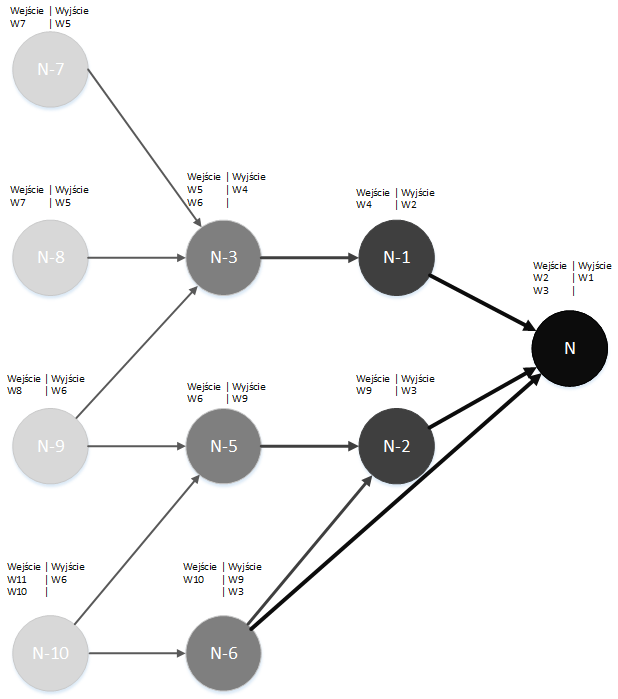
\includegraphics[height=\frameheight]{pictures/visio/siec.png}
 \end{figure}
\end{frame}

\begin{frame}
 \frametitle{Sposób budowy sieci}
 \framesubtitle{Praktyczny przykład}
  \begin{figure}
 		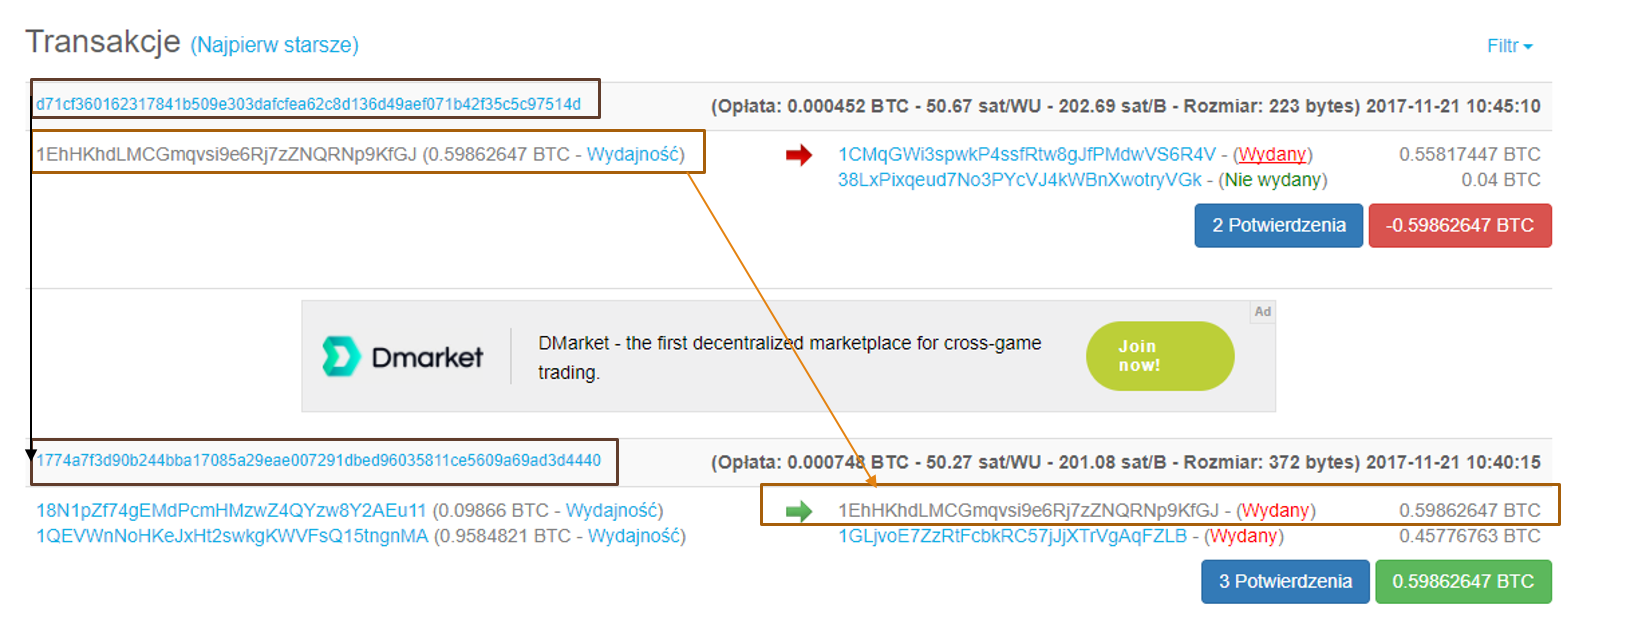
\includegraphics[width=1\linewidth]{pictures/transakcje.png}
	\end{figure}
\end{frame}

\begin{frame}
 \frametitle{Przykładowa sieć}
 \framesubtitle{}
  \begin{figure}
	\centering
 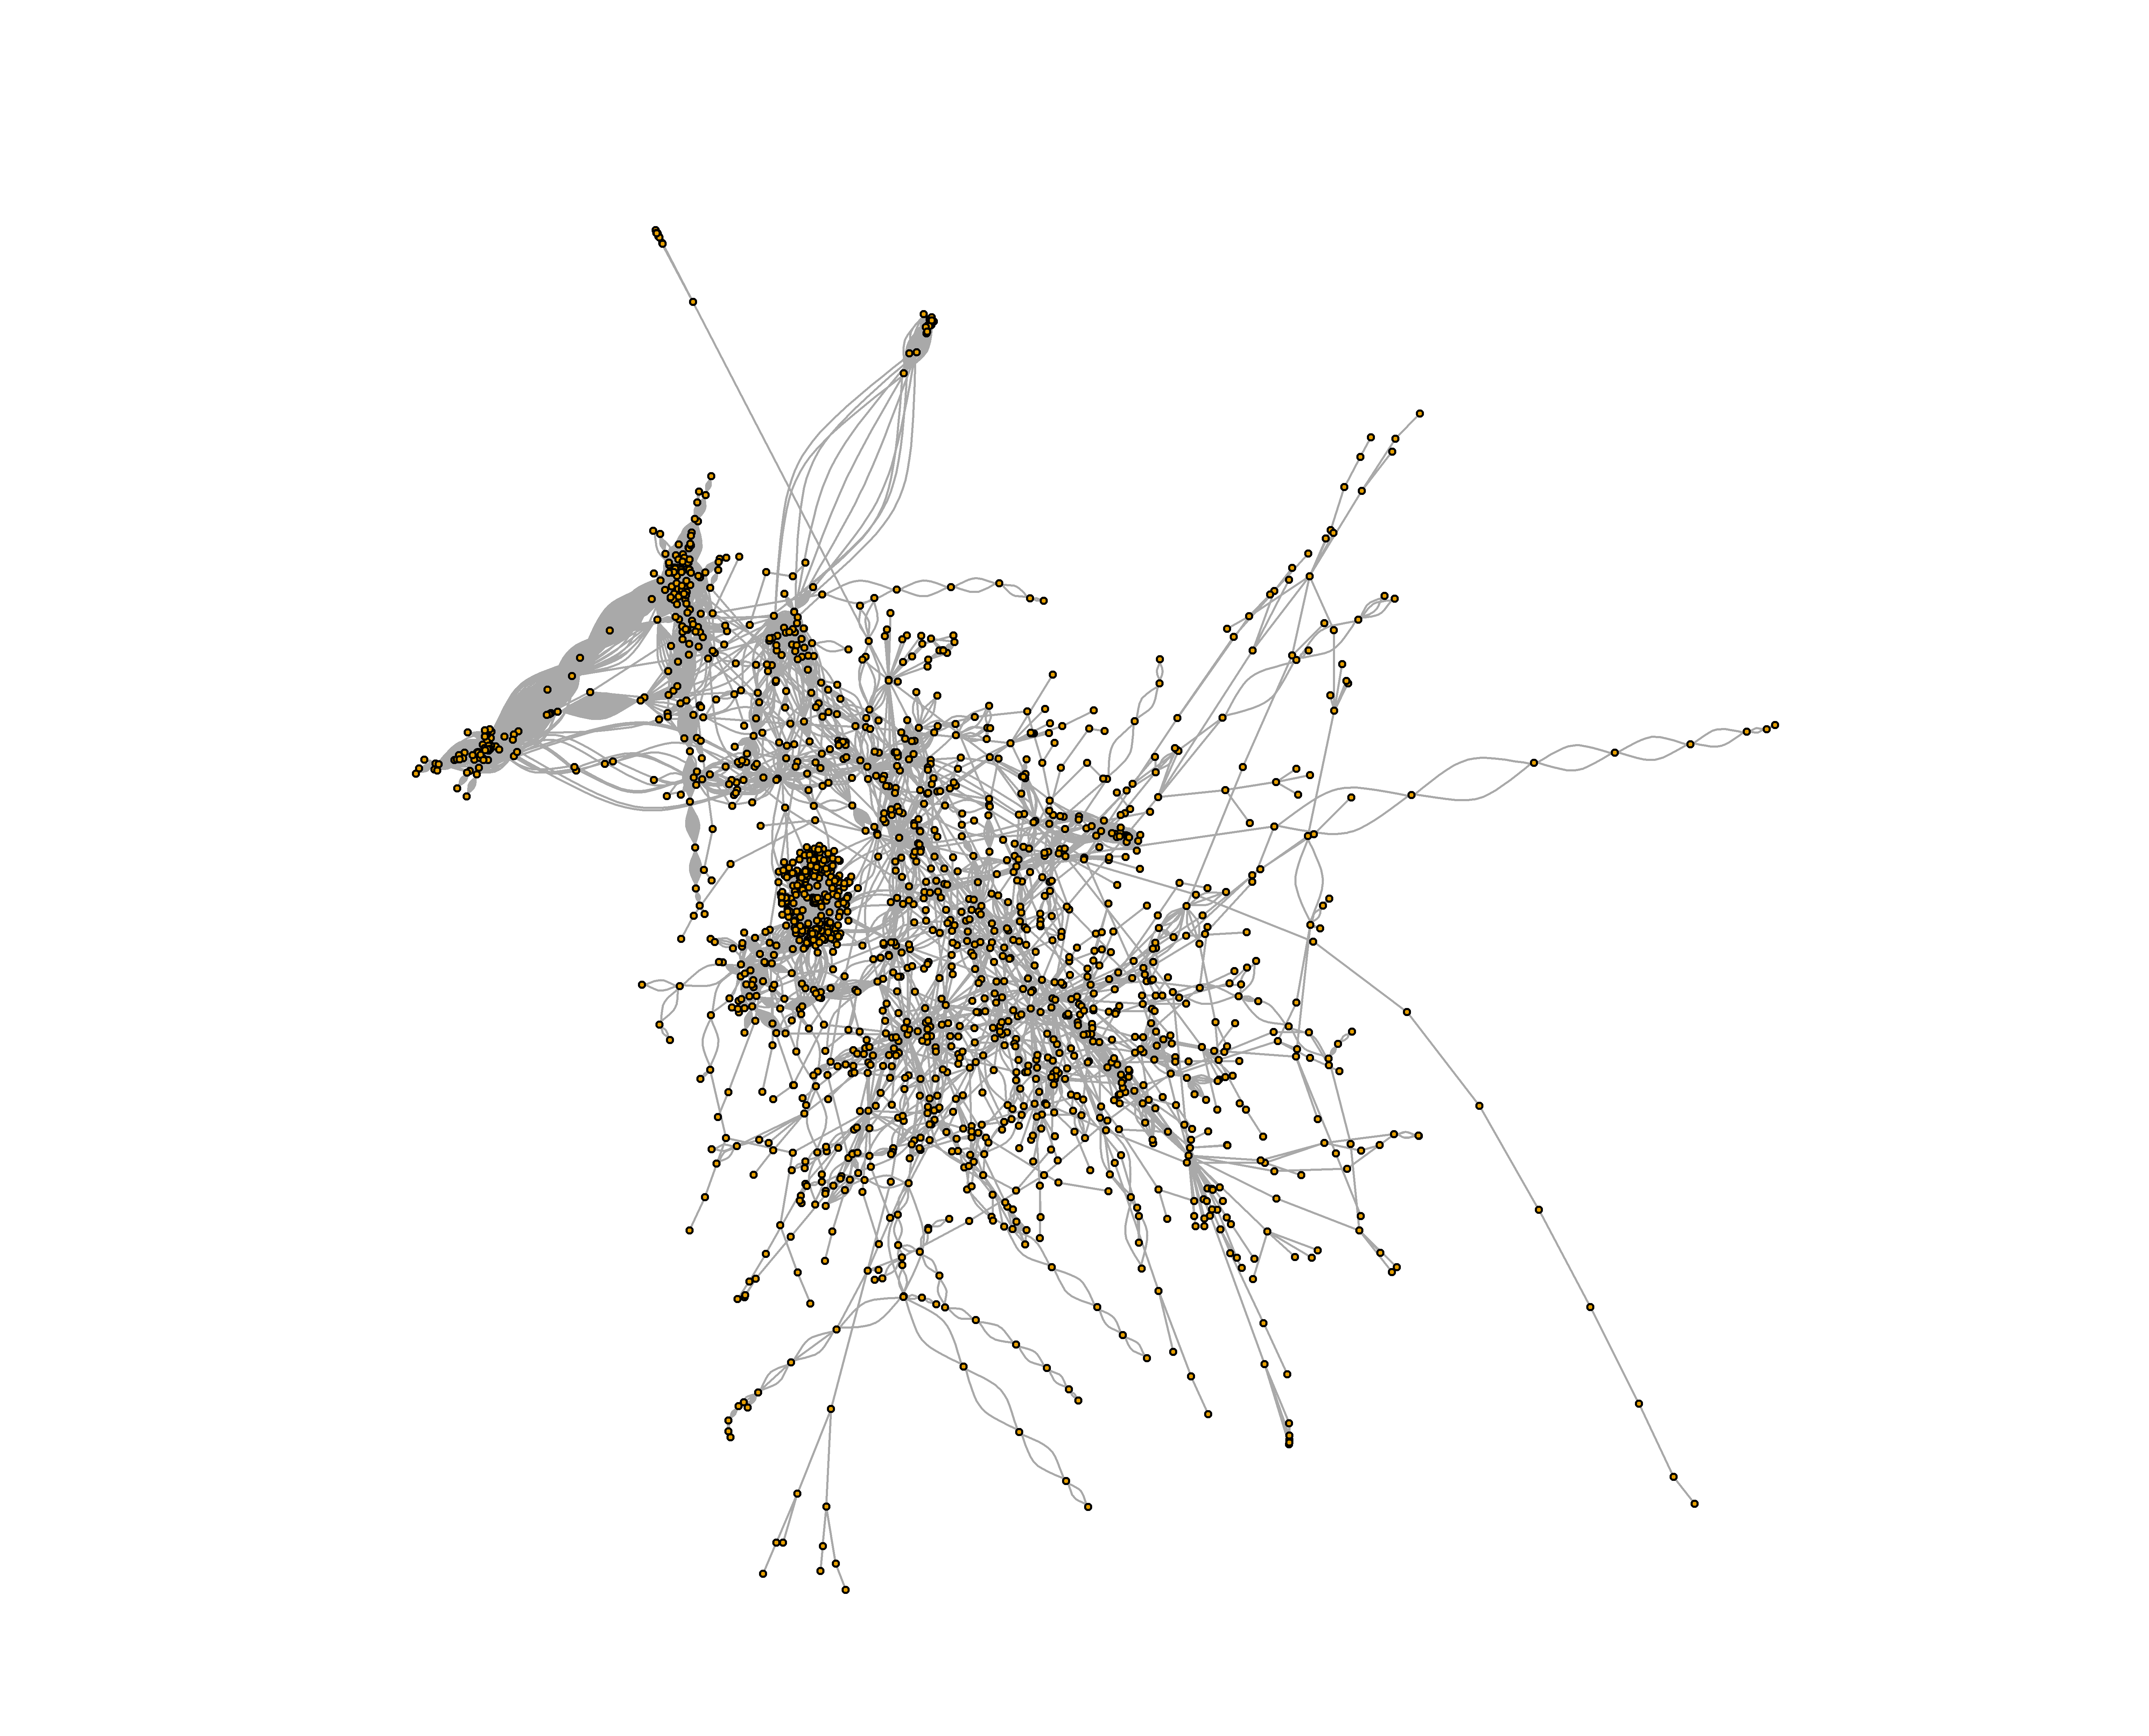
\includegraphics[height=\frameheight]{pictures/graph/graph.png}
  \end{figure}
\end{frame}


\begin{frame}
 \frametitle{Przeprowadzone badania}
 \framesubtitle{}
 \justify
Przeprowadzono badania podstawowych właściwości sieci:
\begin{itemize}
\item średnicy,
\item średniej długości ścieżek,
\item średniego stopienia węzłów,
\item średniej centralności węzłów,
\end{itemize}
oraz badania wynikające z jej specyfiki:
\begin{itemize}
\item średnia wartość transakcji,
\item liczba bloków potrzebnych do stworzenia próby,
\item średnia różnica czasów kolejnych transakcji,
\item różnica czasu granicznych transakcji.
\end{itemize}
\end{frame}

\begin{frame}
 \frametitle{Wyniki}
 \framesubtitle{Generyczne właściwości sieci}
  \begin{minipage}{\textwidth}
     \centering
 			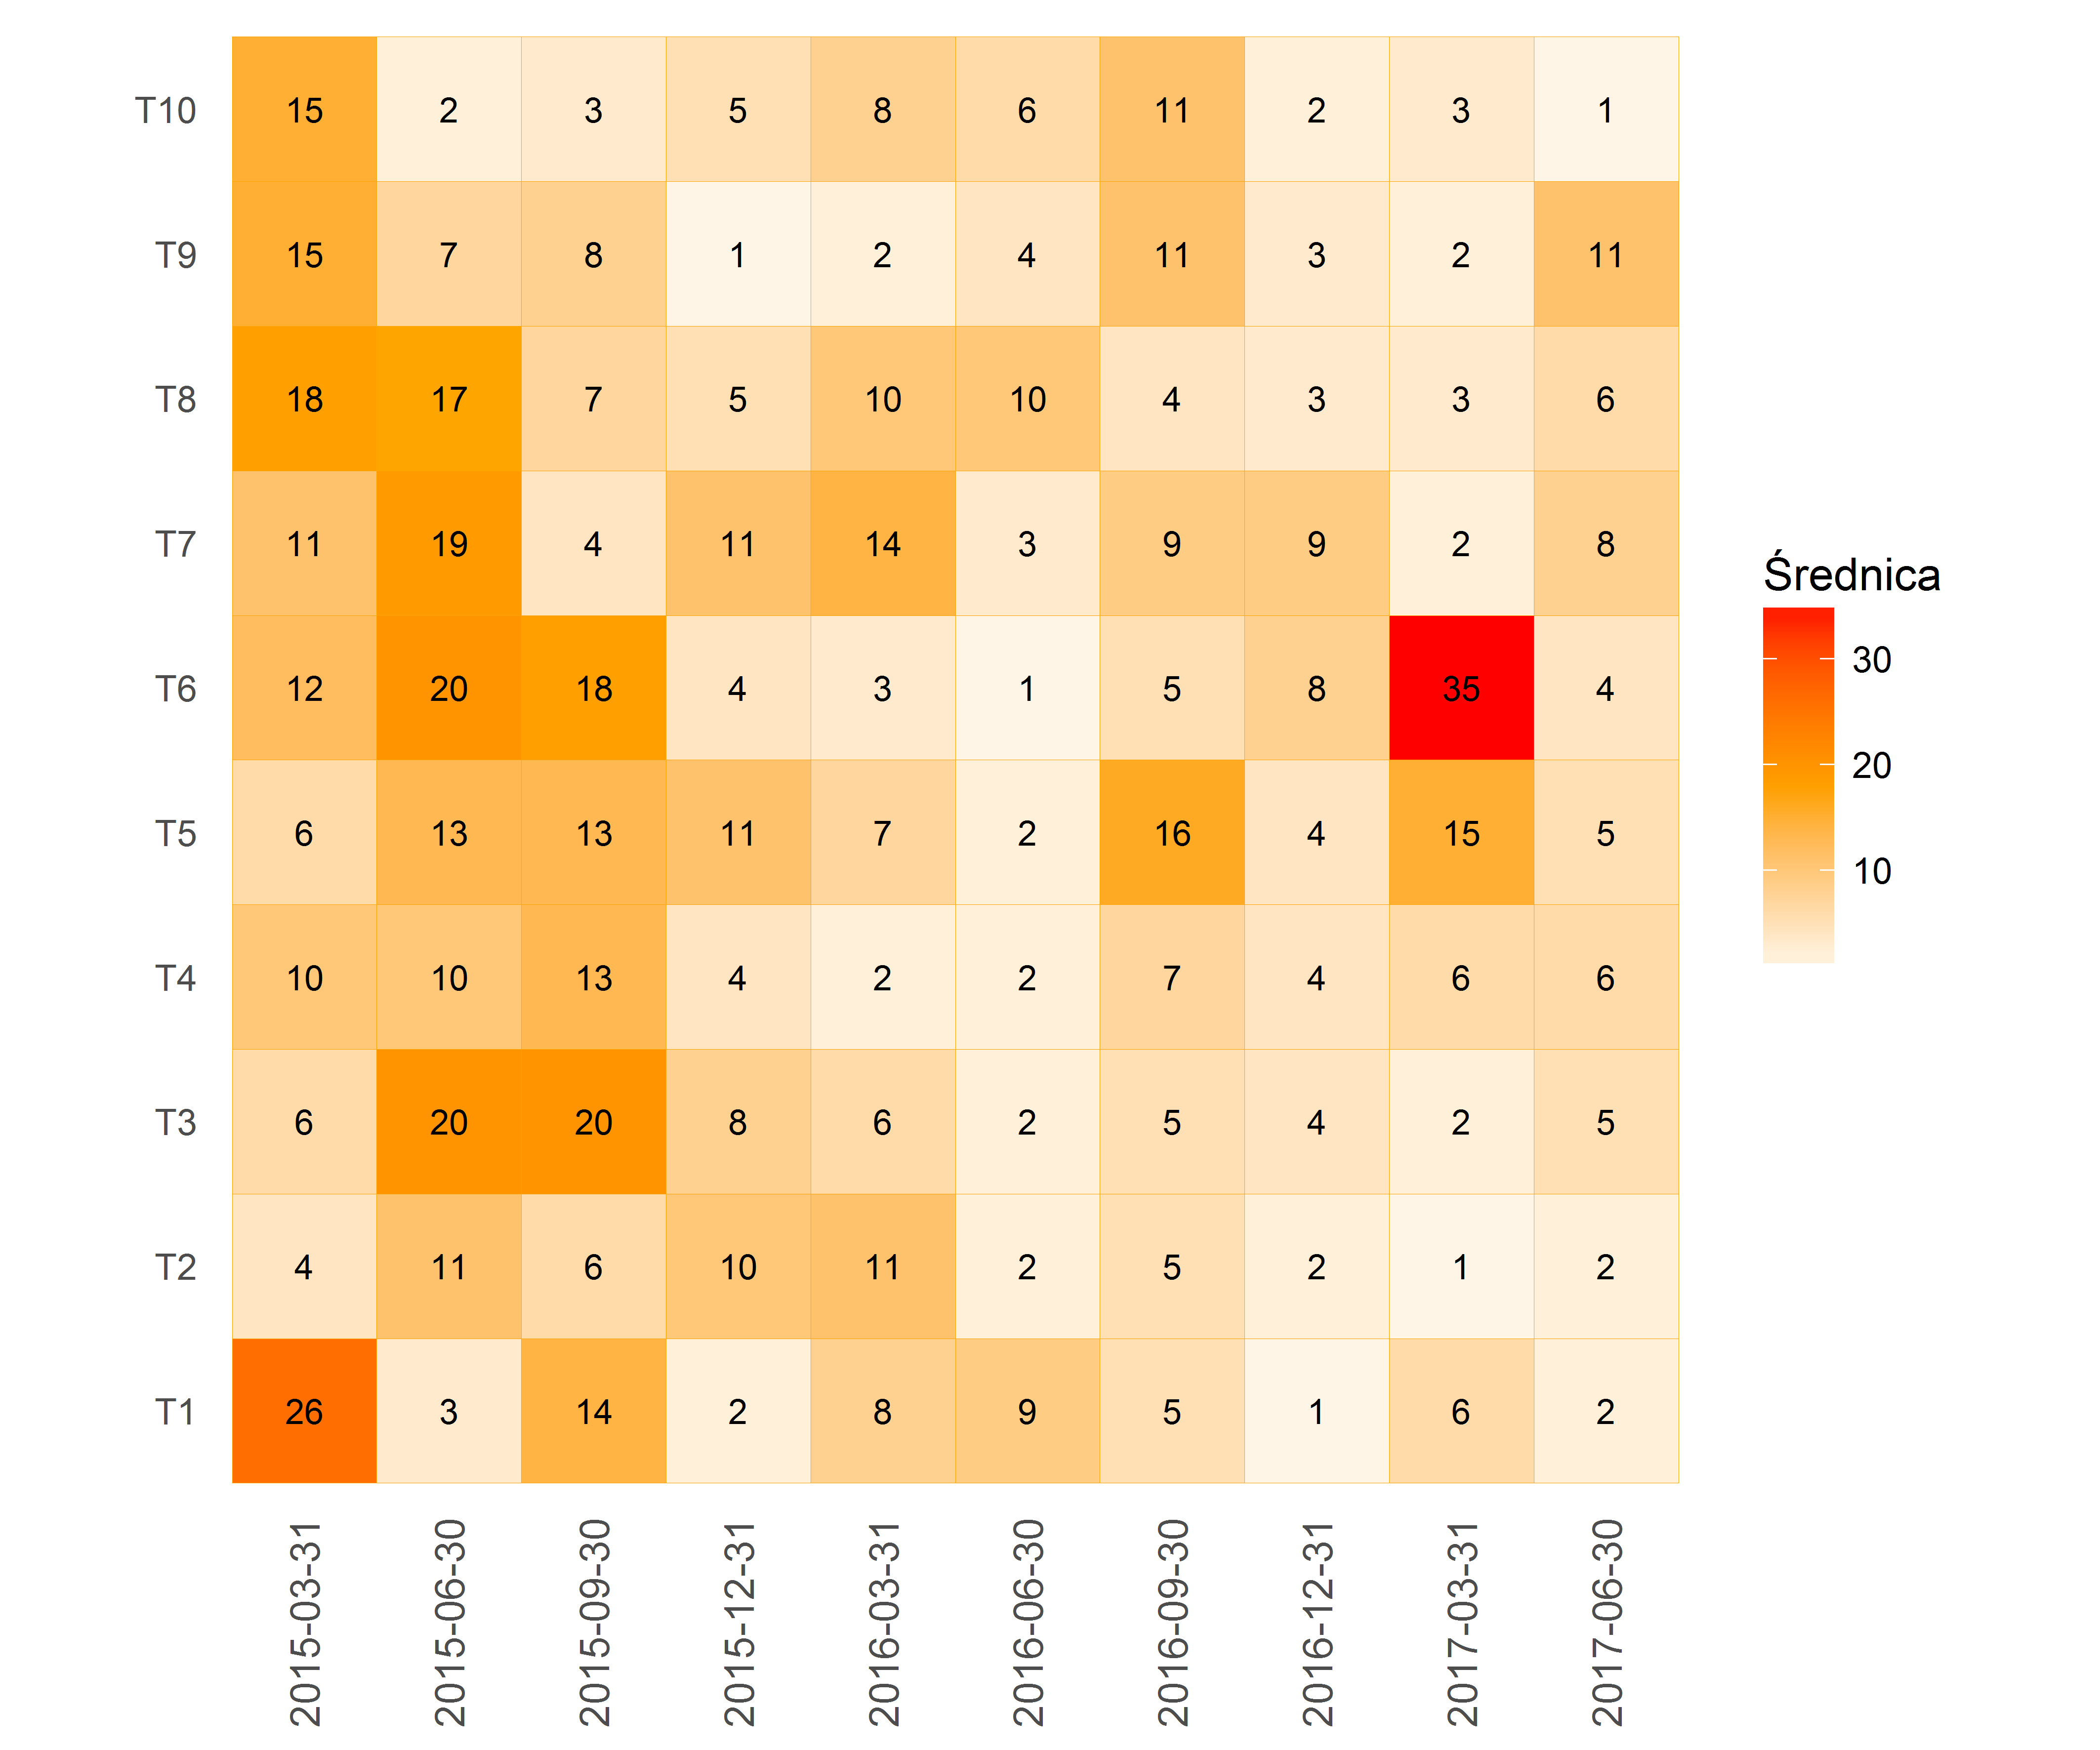
\includegraphics[width=\sizequad\textwidth]{pictures/srednica/srednica_hm.png}\quad  
            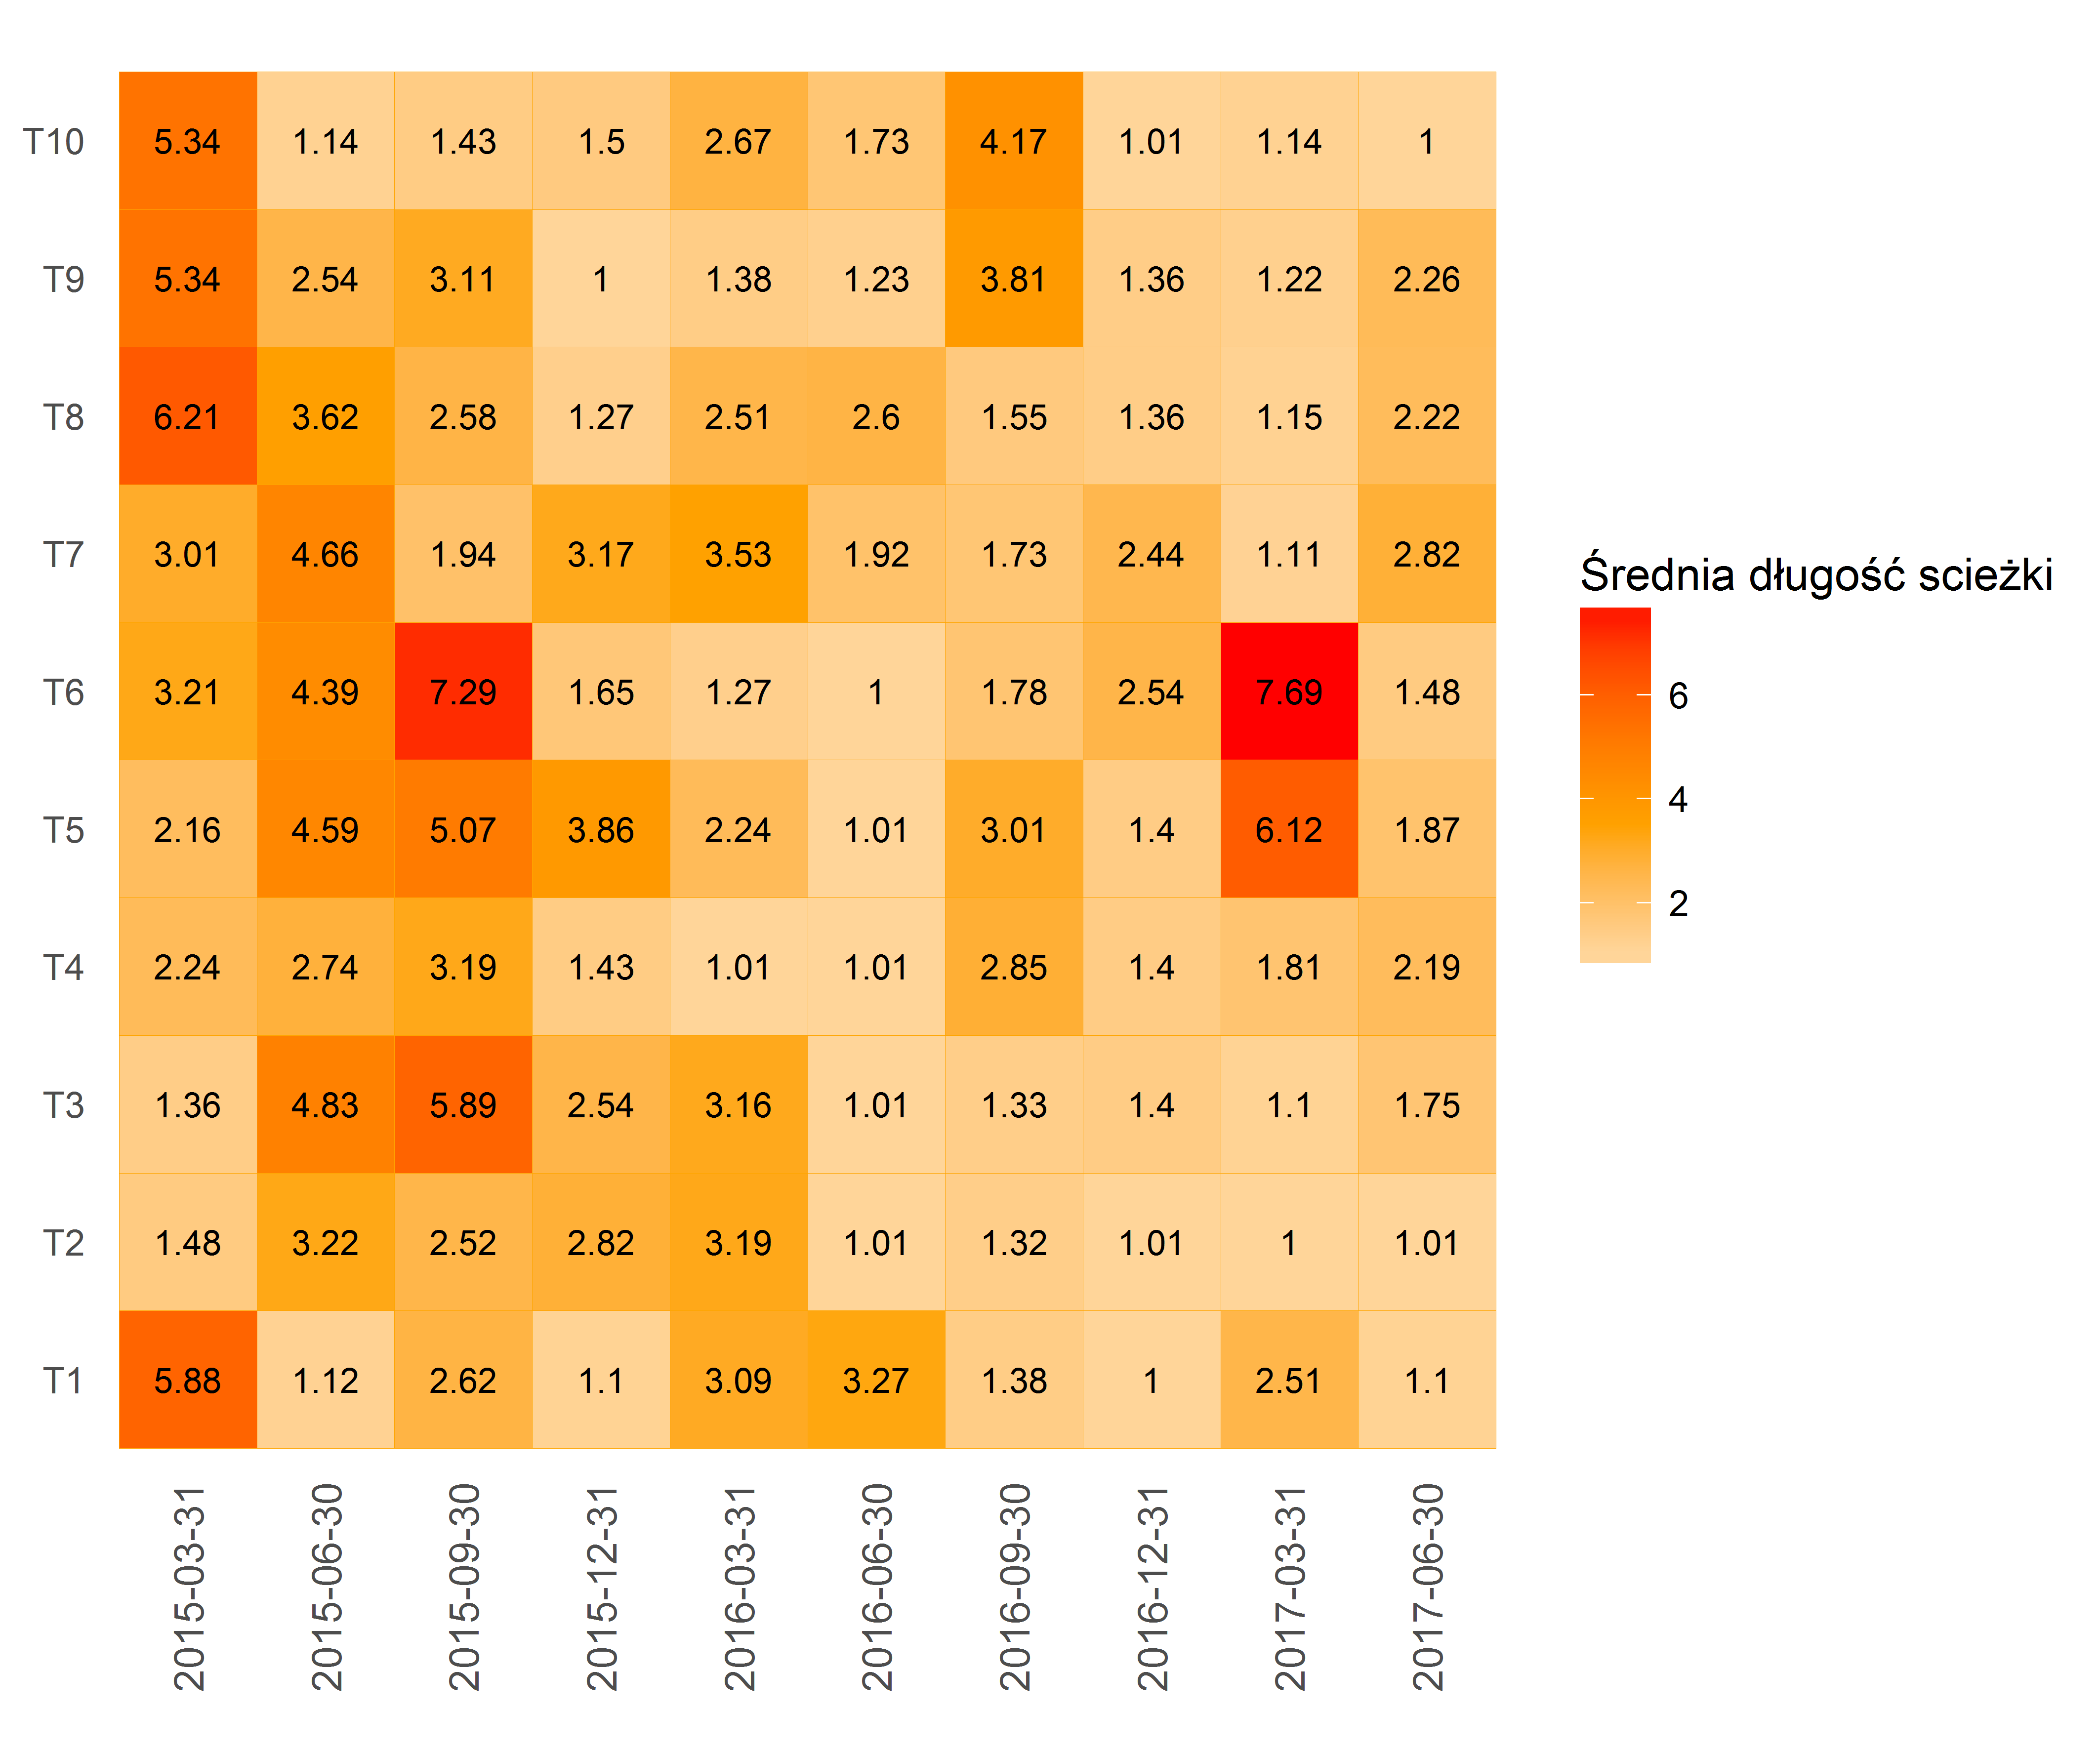
\includegraphics[width=\sizequad\textwidth]{pictures/srednia_dlugosc_sciezki/srednia_dlugosc_sciezki_hm.png}  \\
            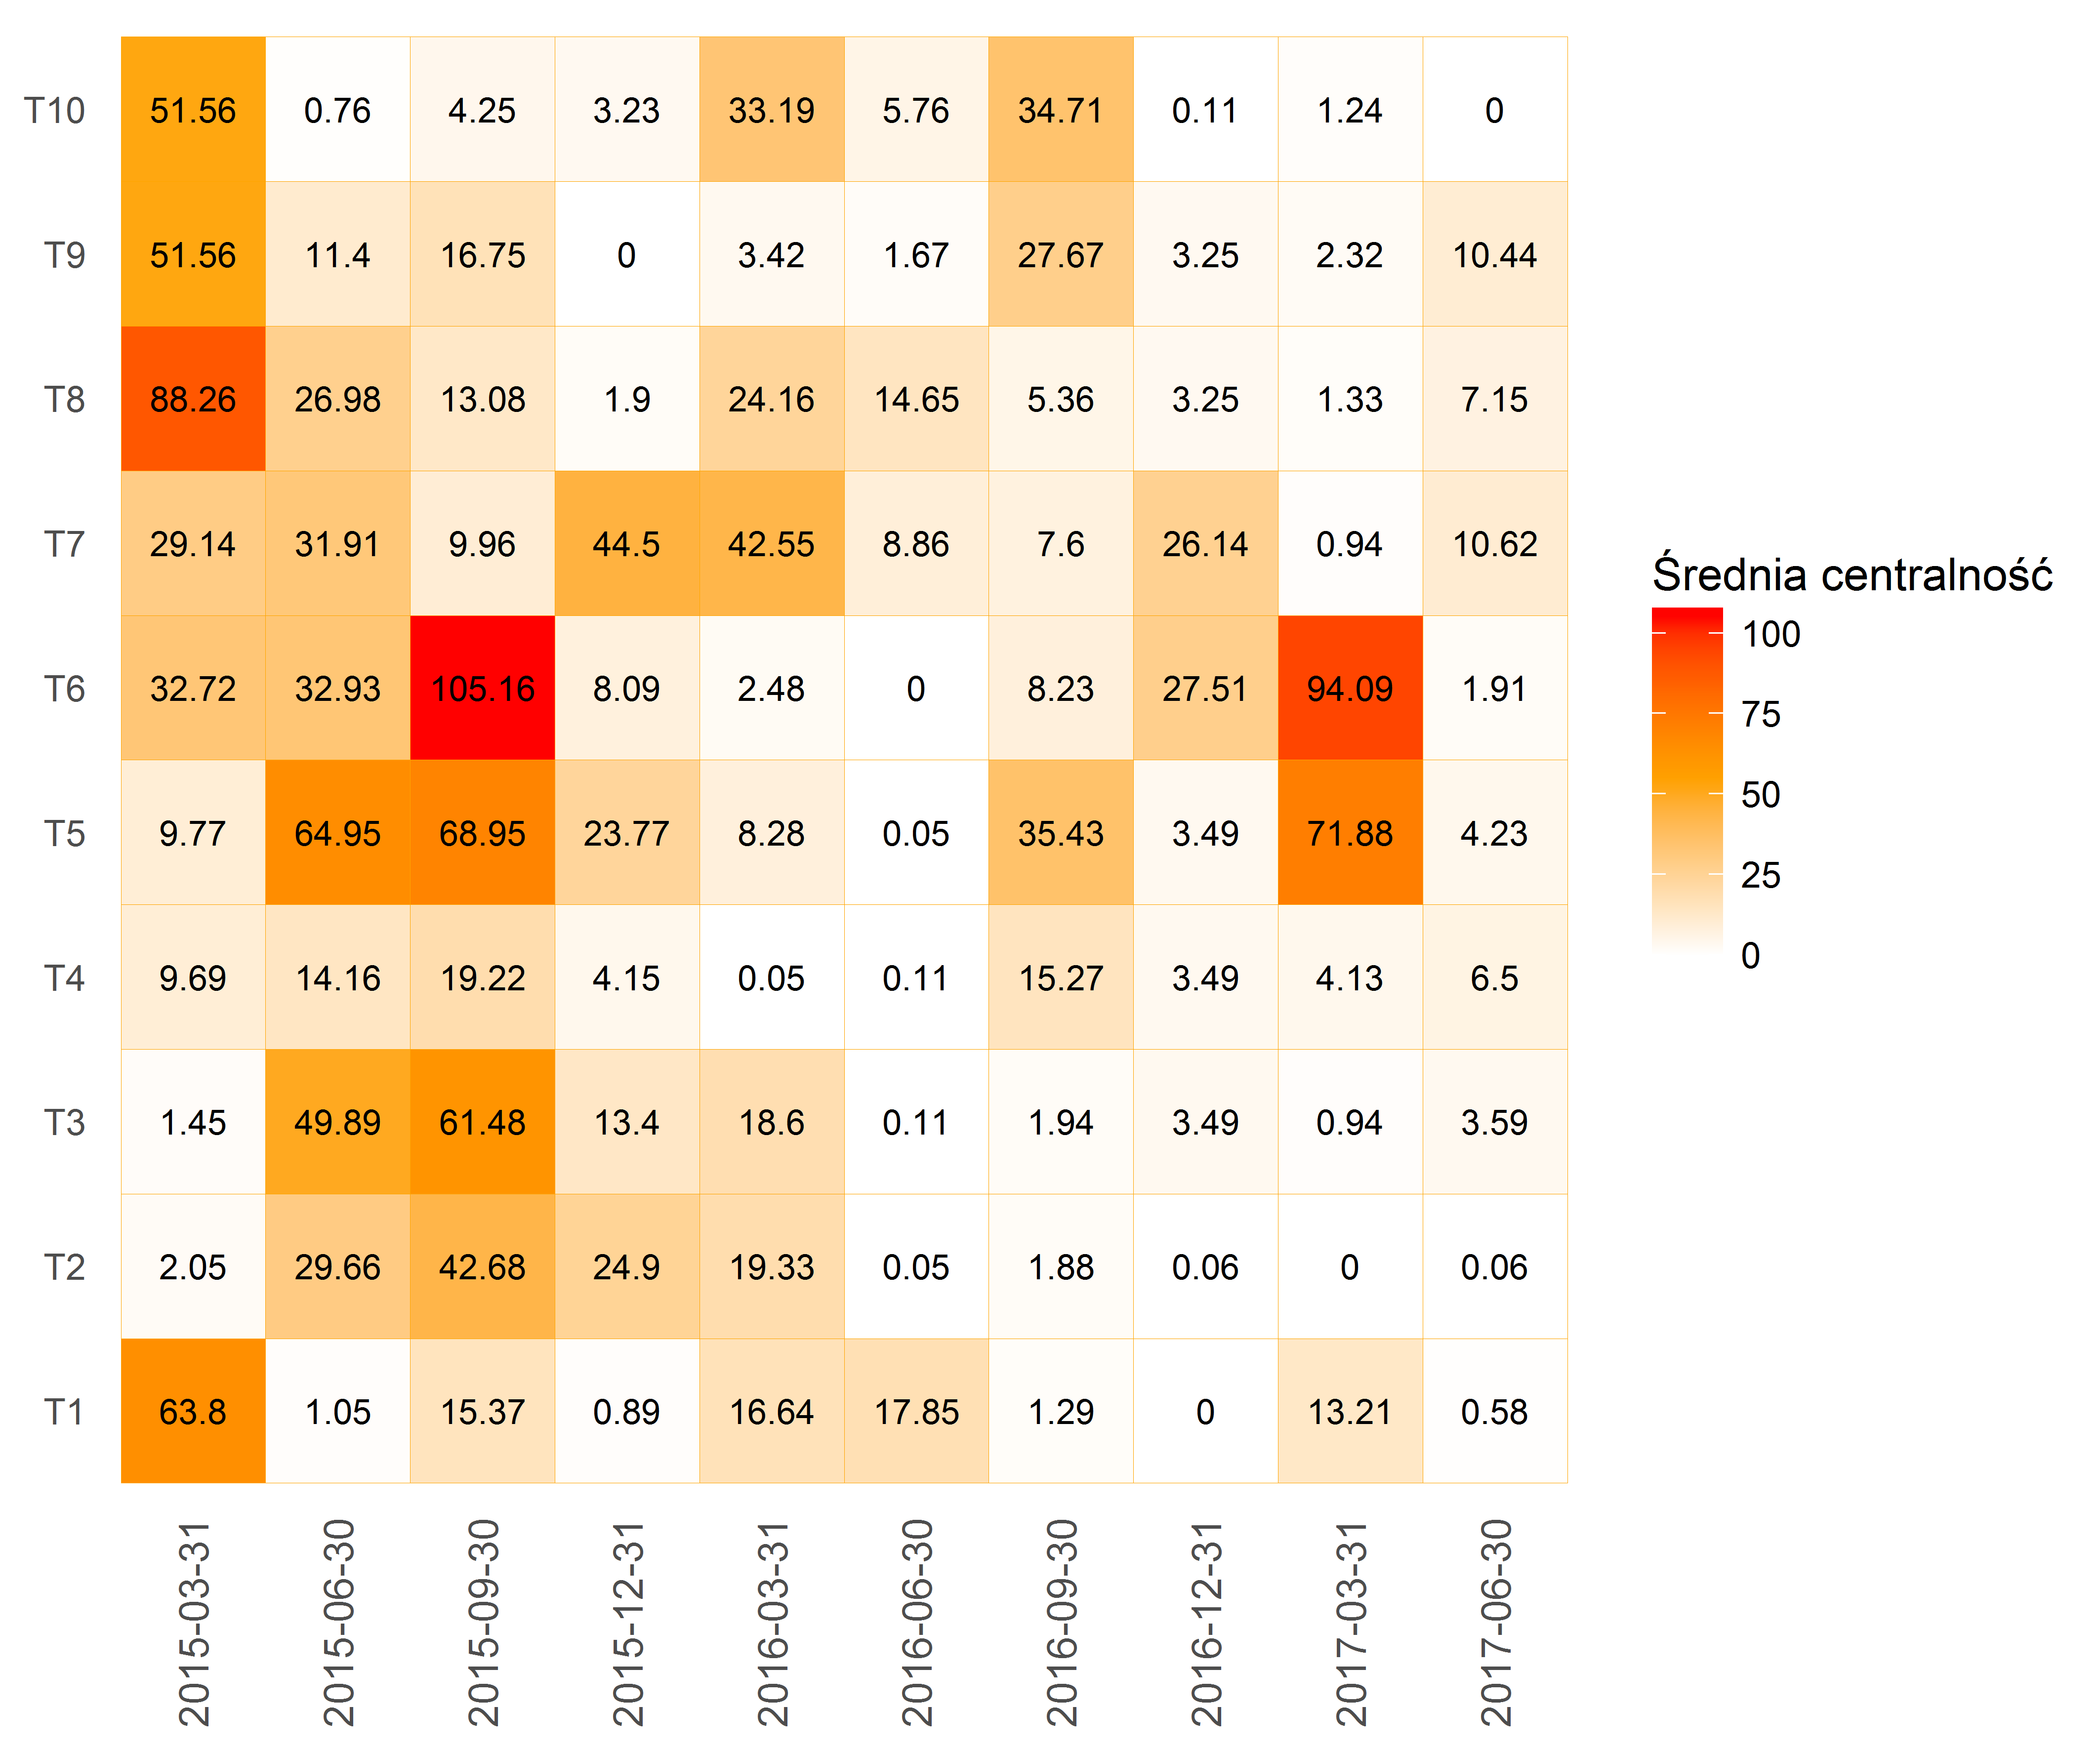
\includegraphics[width=\sizequad\textwidth]{pictures/srednia_centralnosc/srednia_centralnosc_hm.png}\quad
			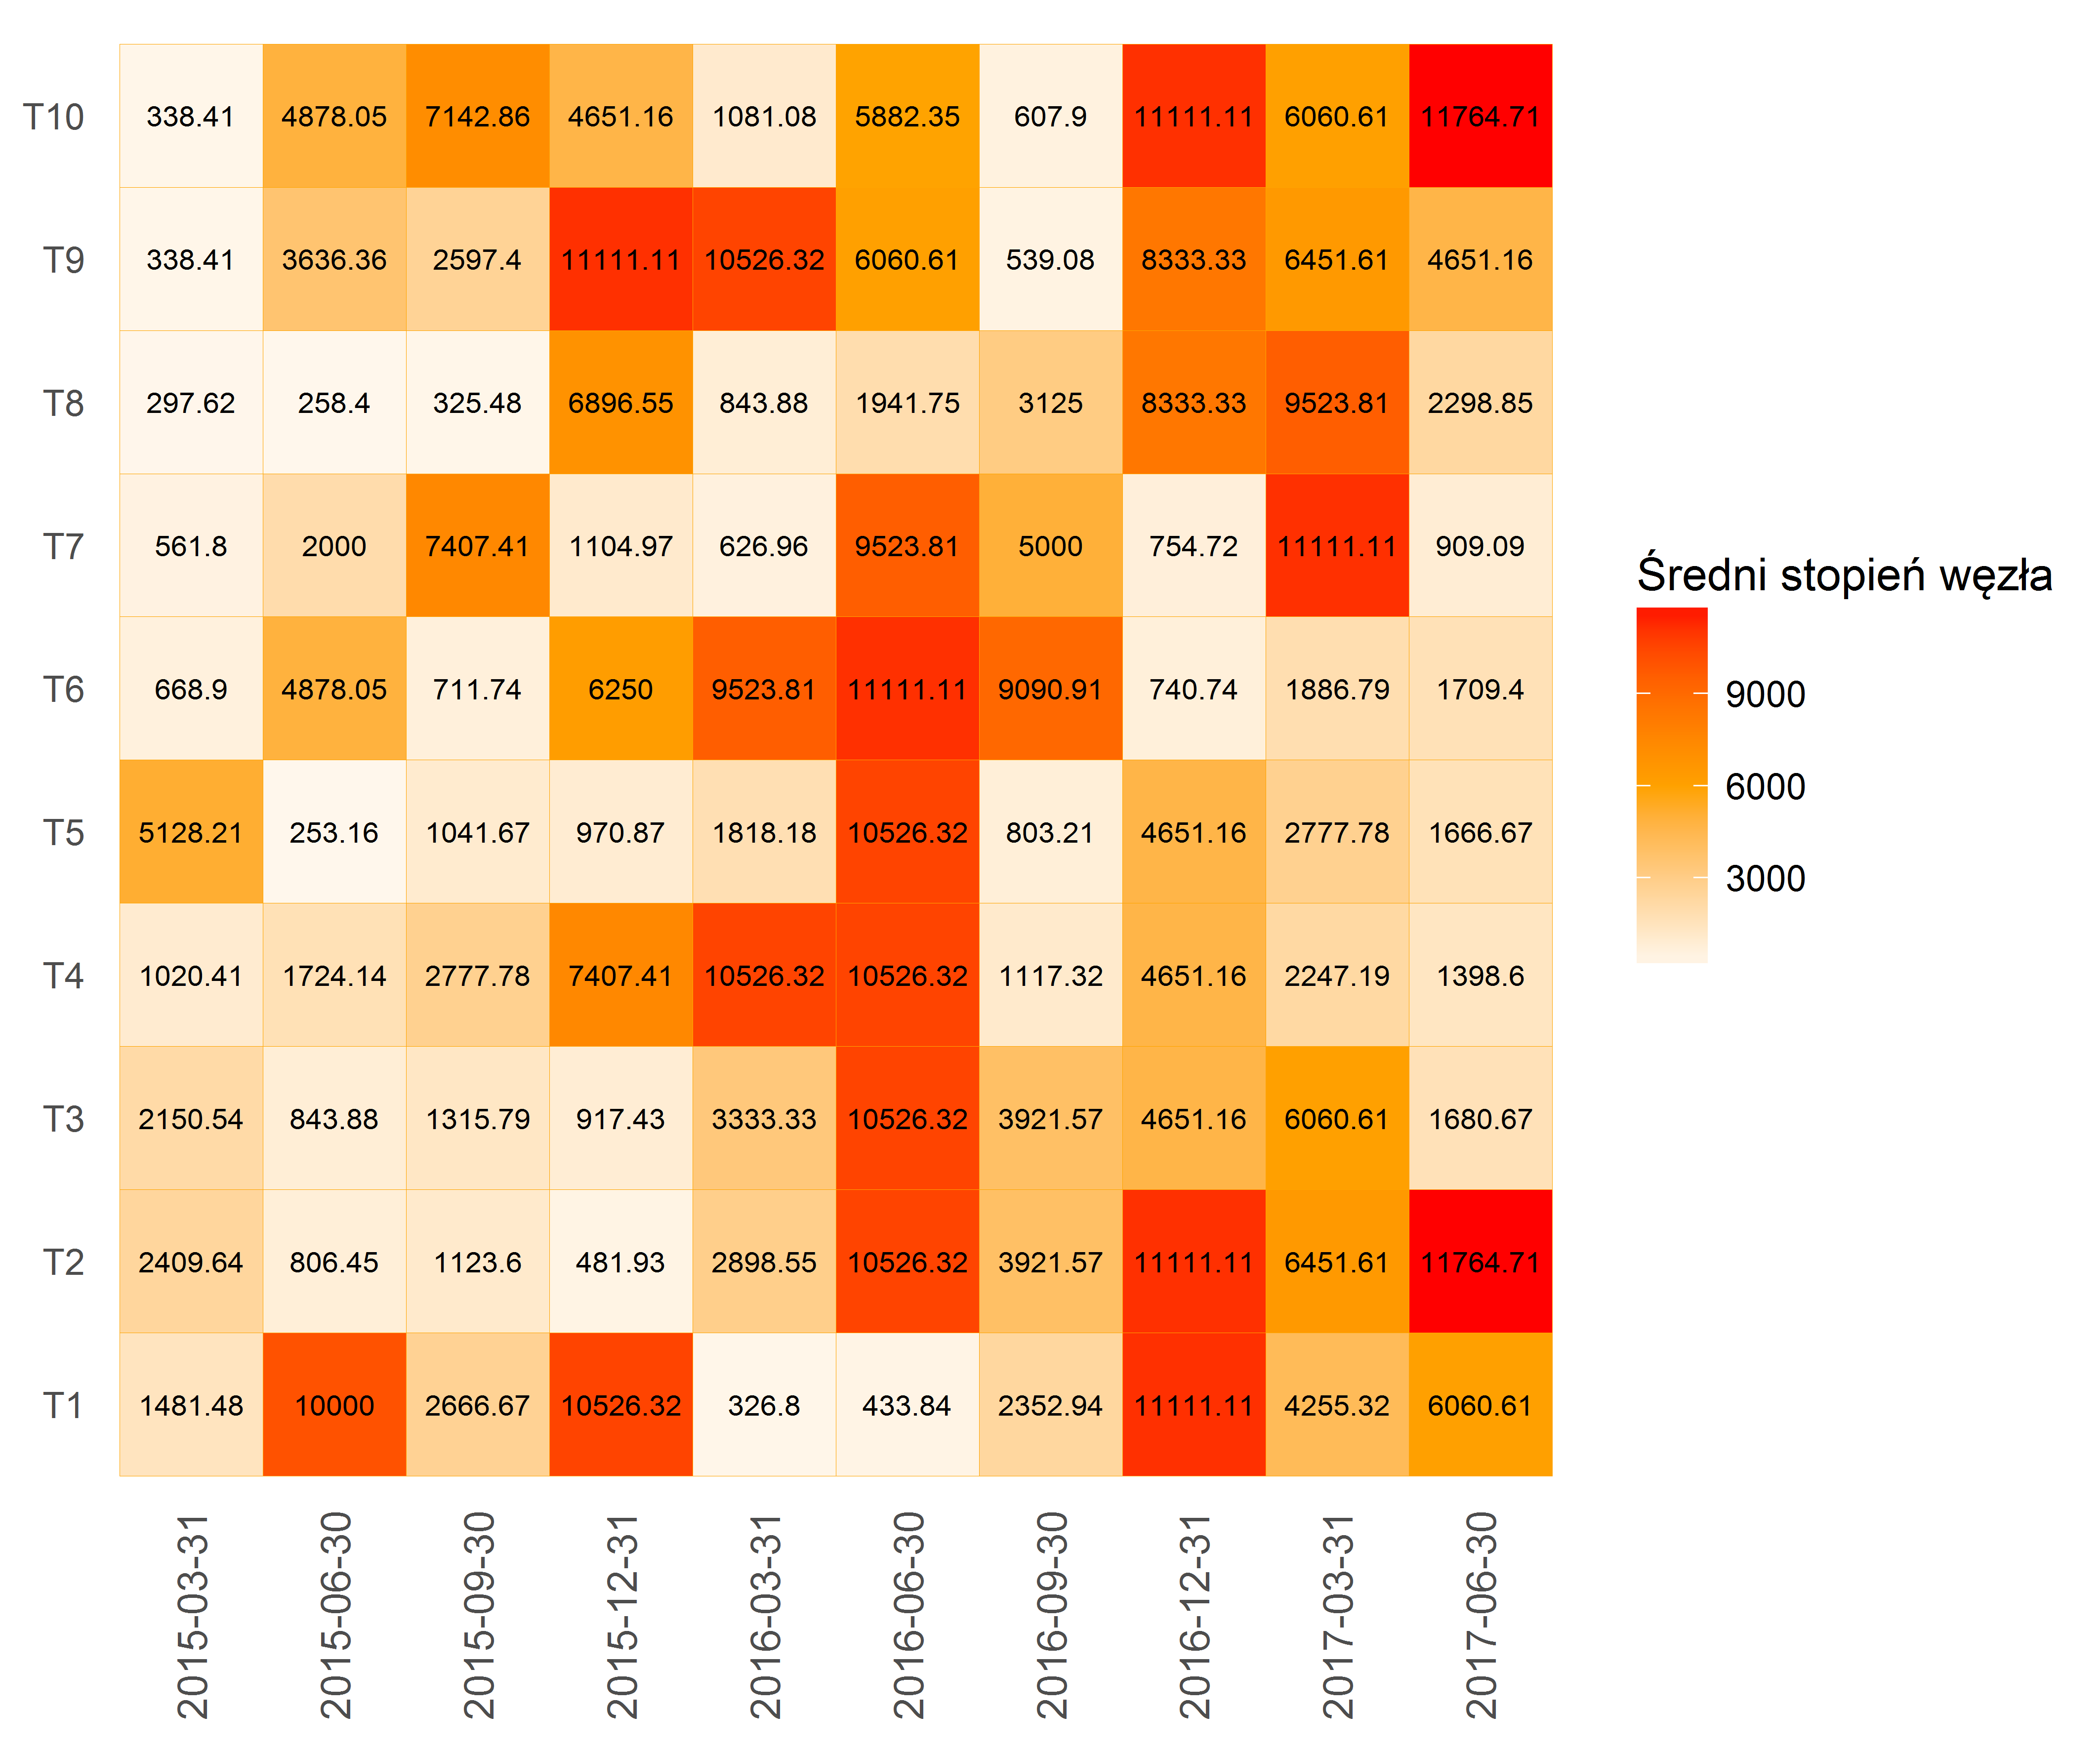
\includegraphics[width=\sizequad\textwidth]{pictures/sredni_stopien_wezla/sredni_stopien_wezla_hm.png}
 \end{minipage} 
 
\end{frame}

\begin{frame}
 \frametitle{Trend}
 \framesubtitle{Generyczne właściwości sieci}
 
  \begin{minipage}{\textwidth}
     \centering
 			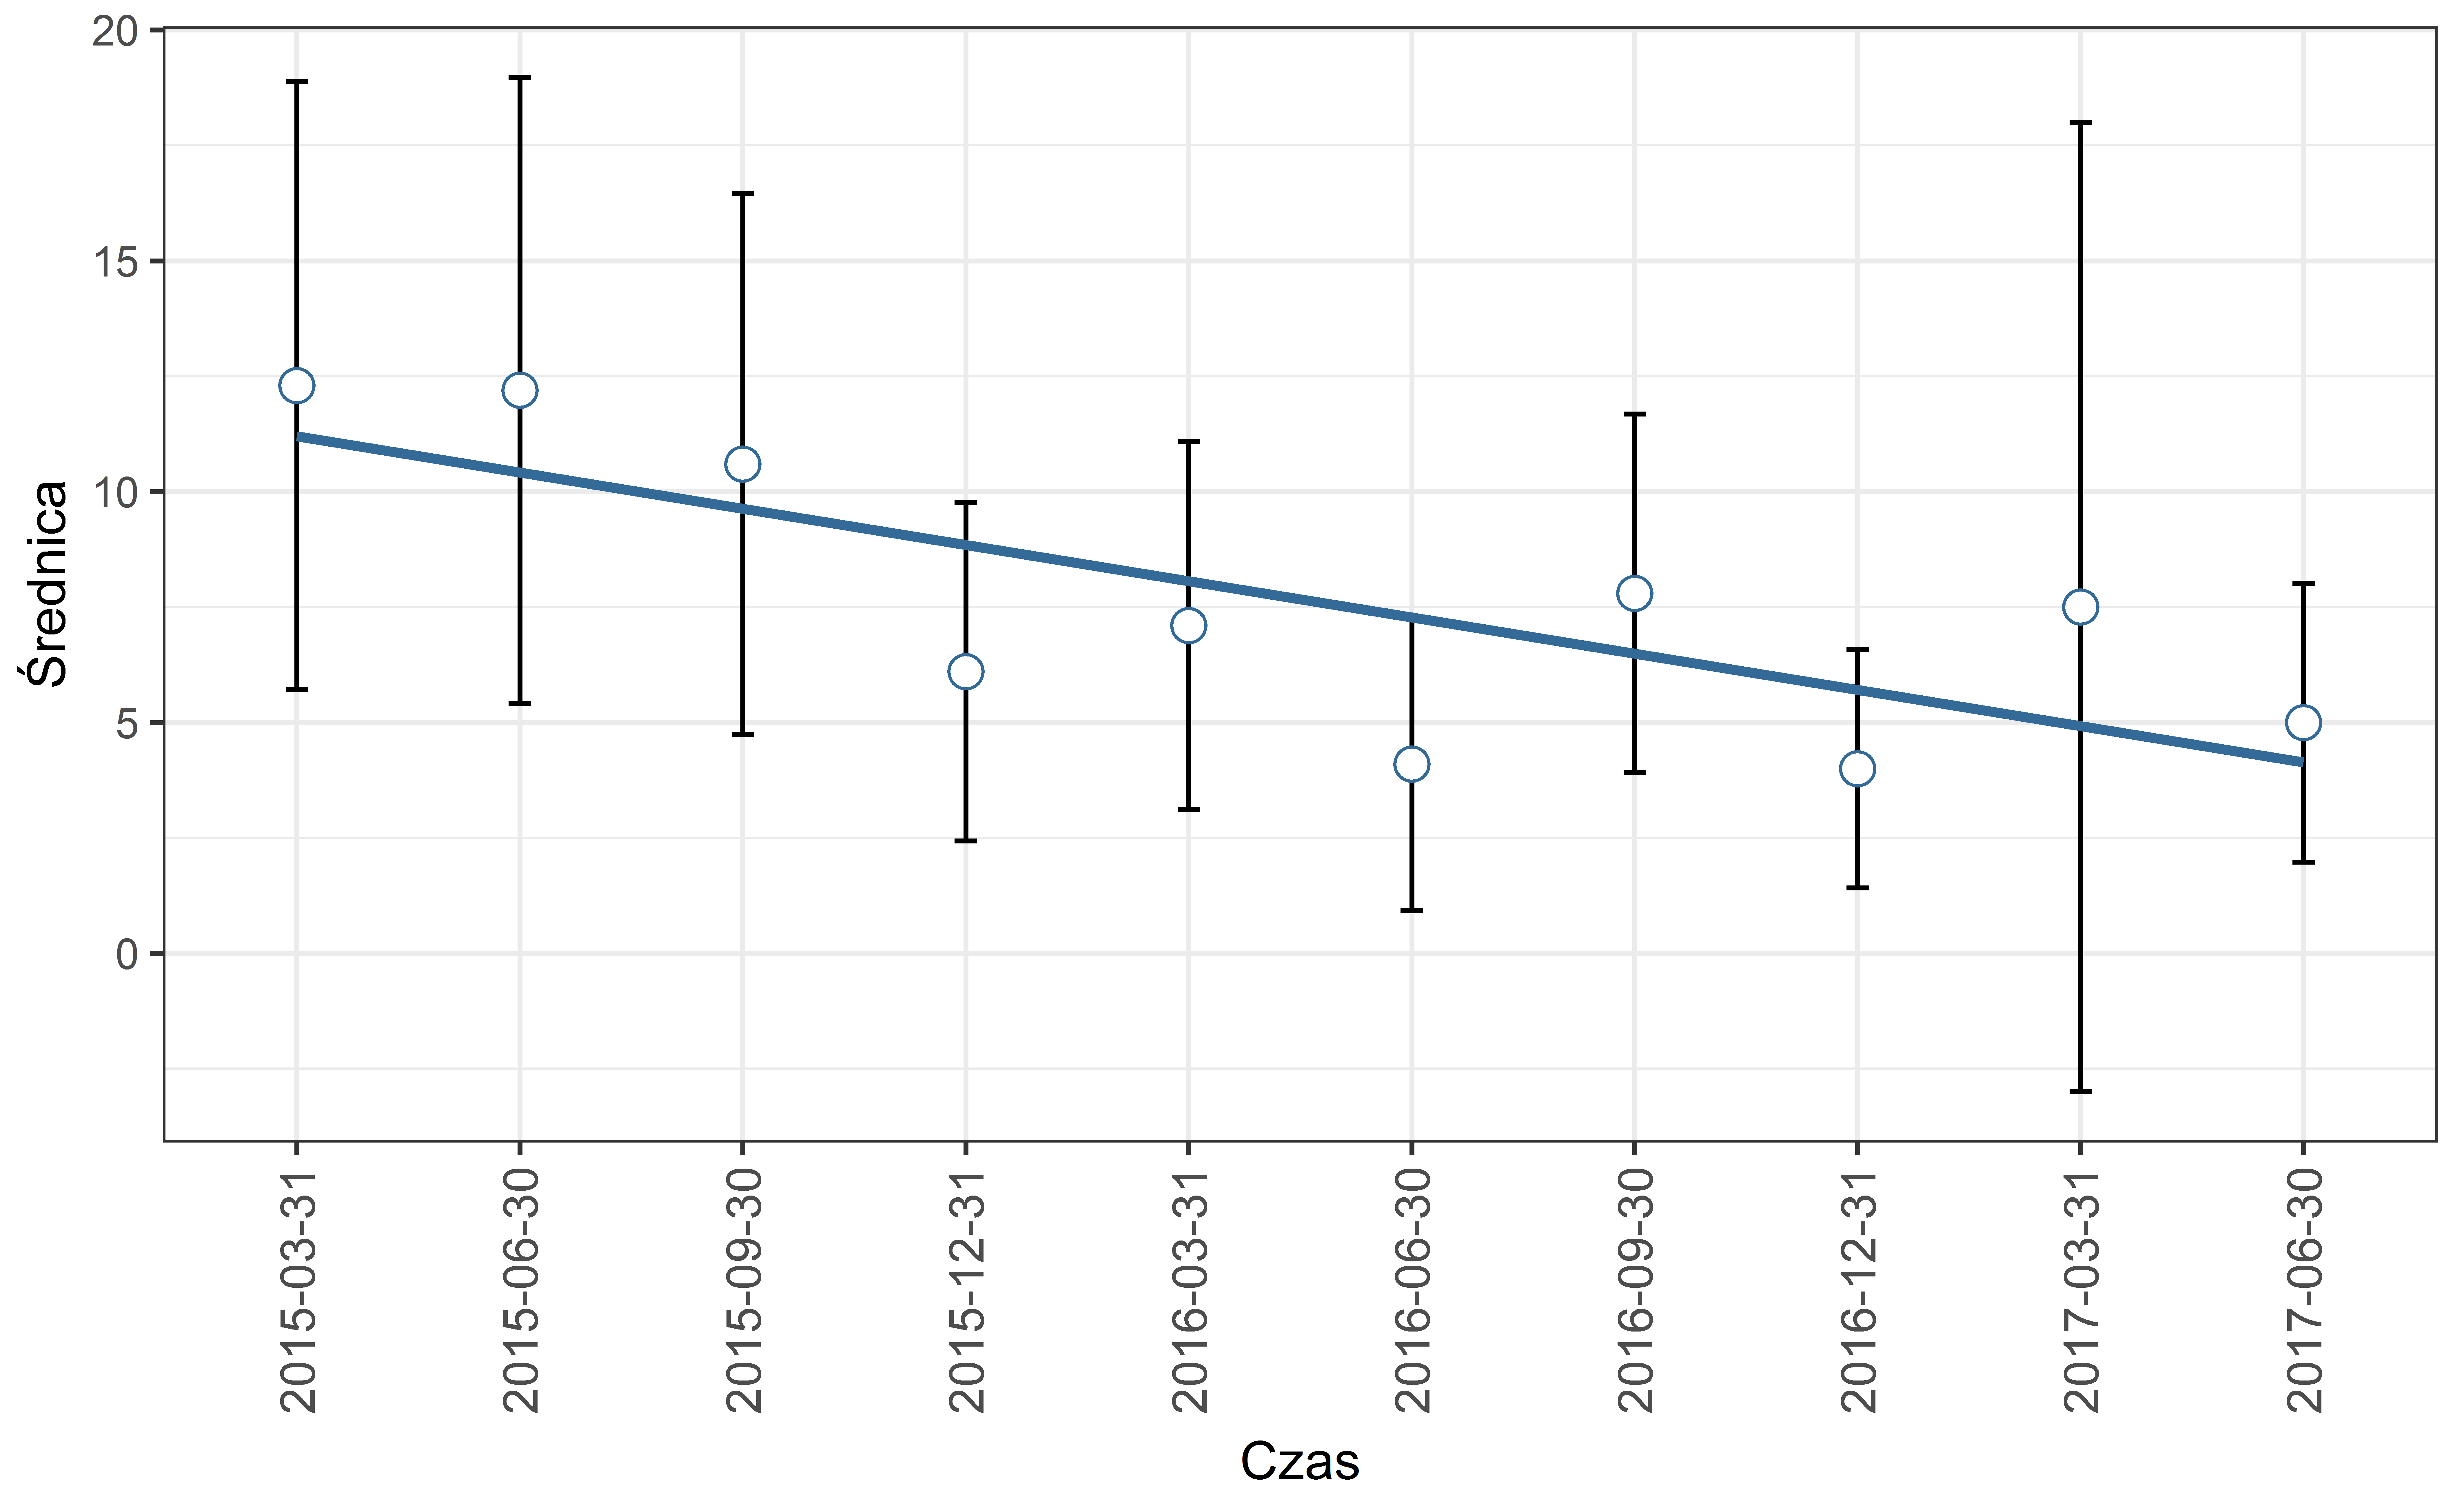
\includegraphics[width=\sizequadsda\textwidth]{pictures/srednica/srednica_sda.png}\quad  
            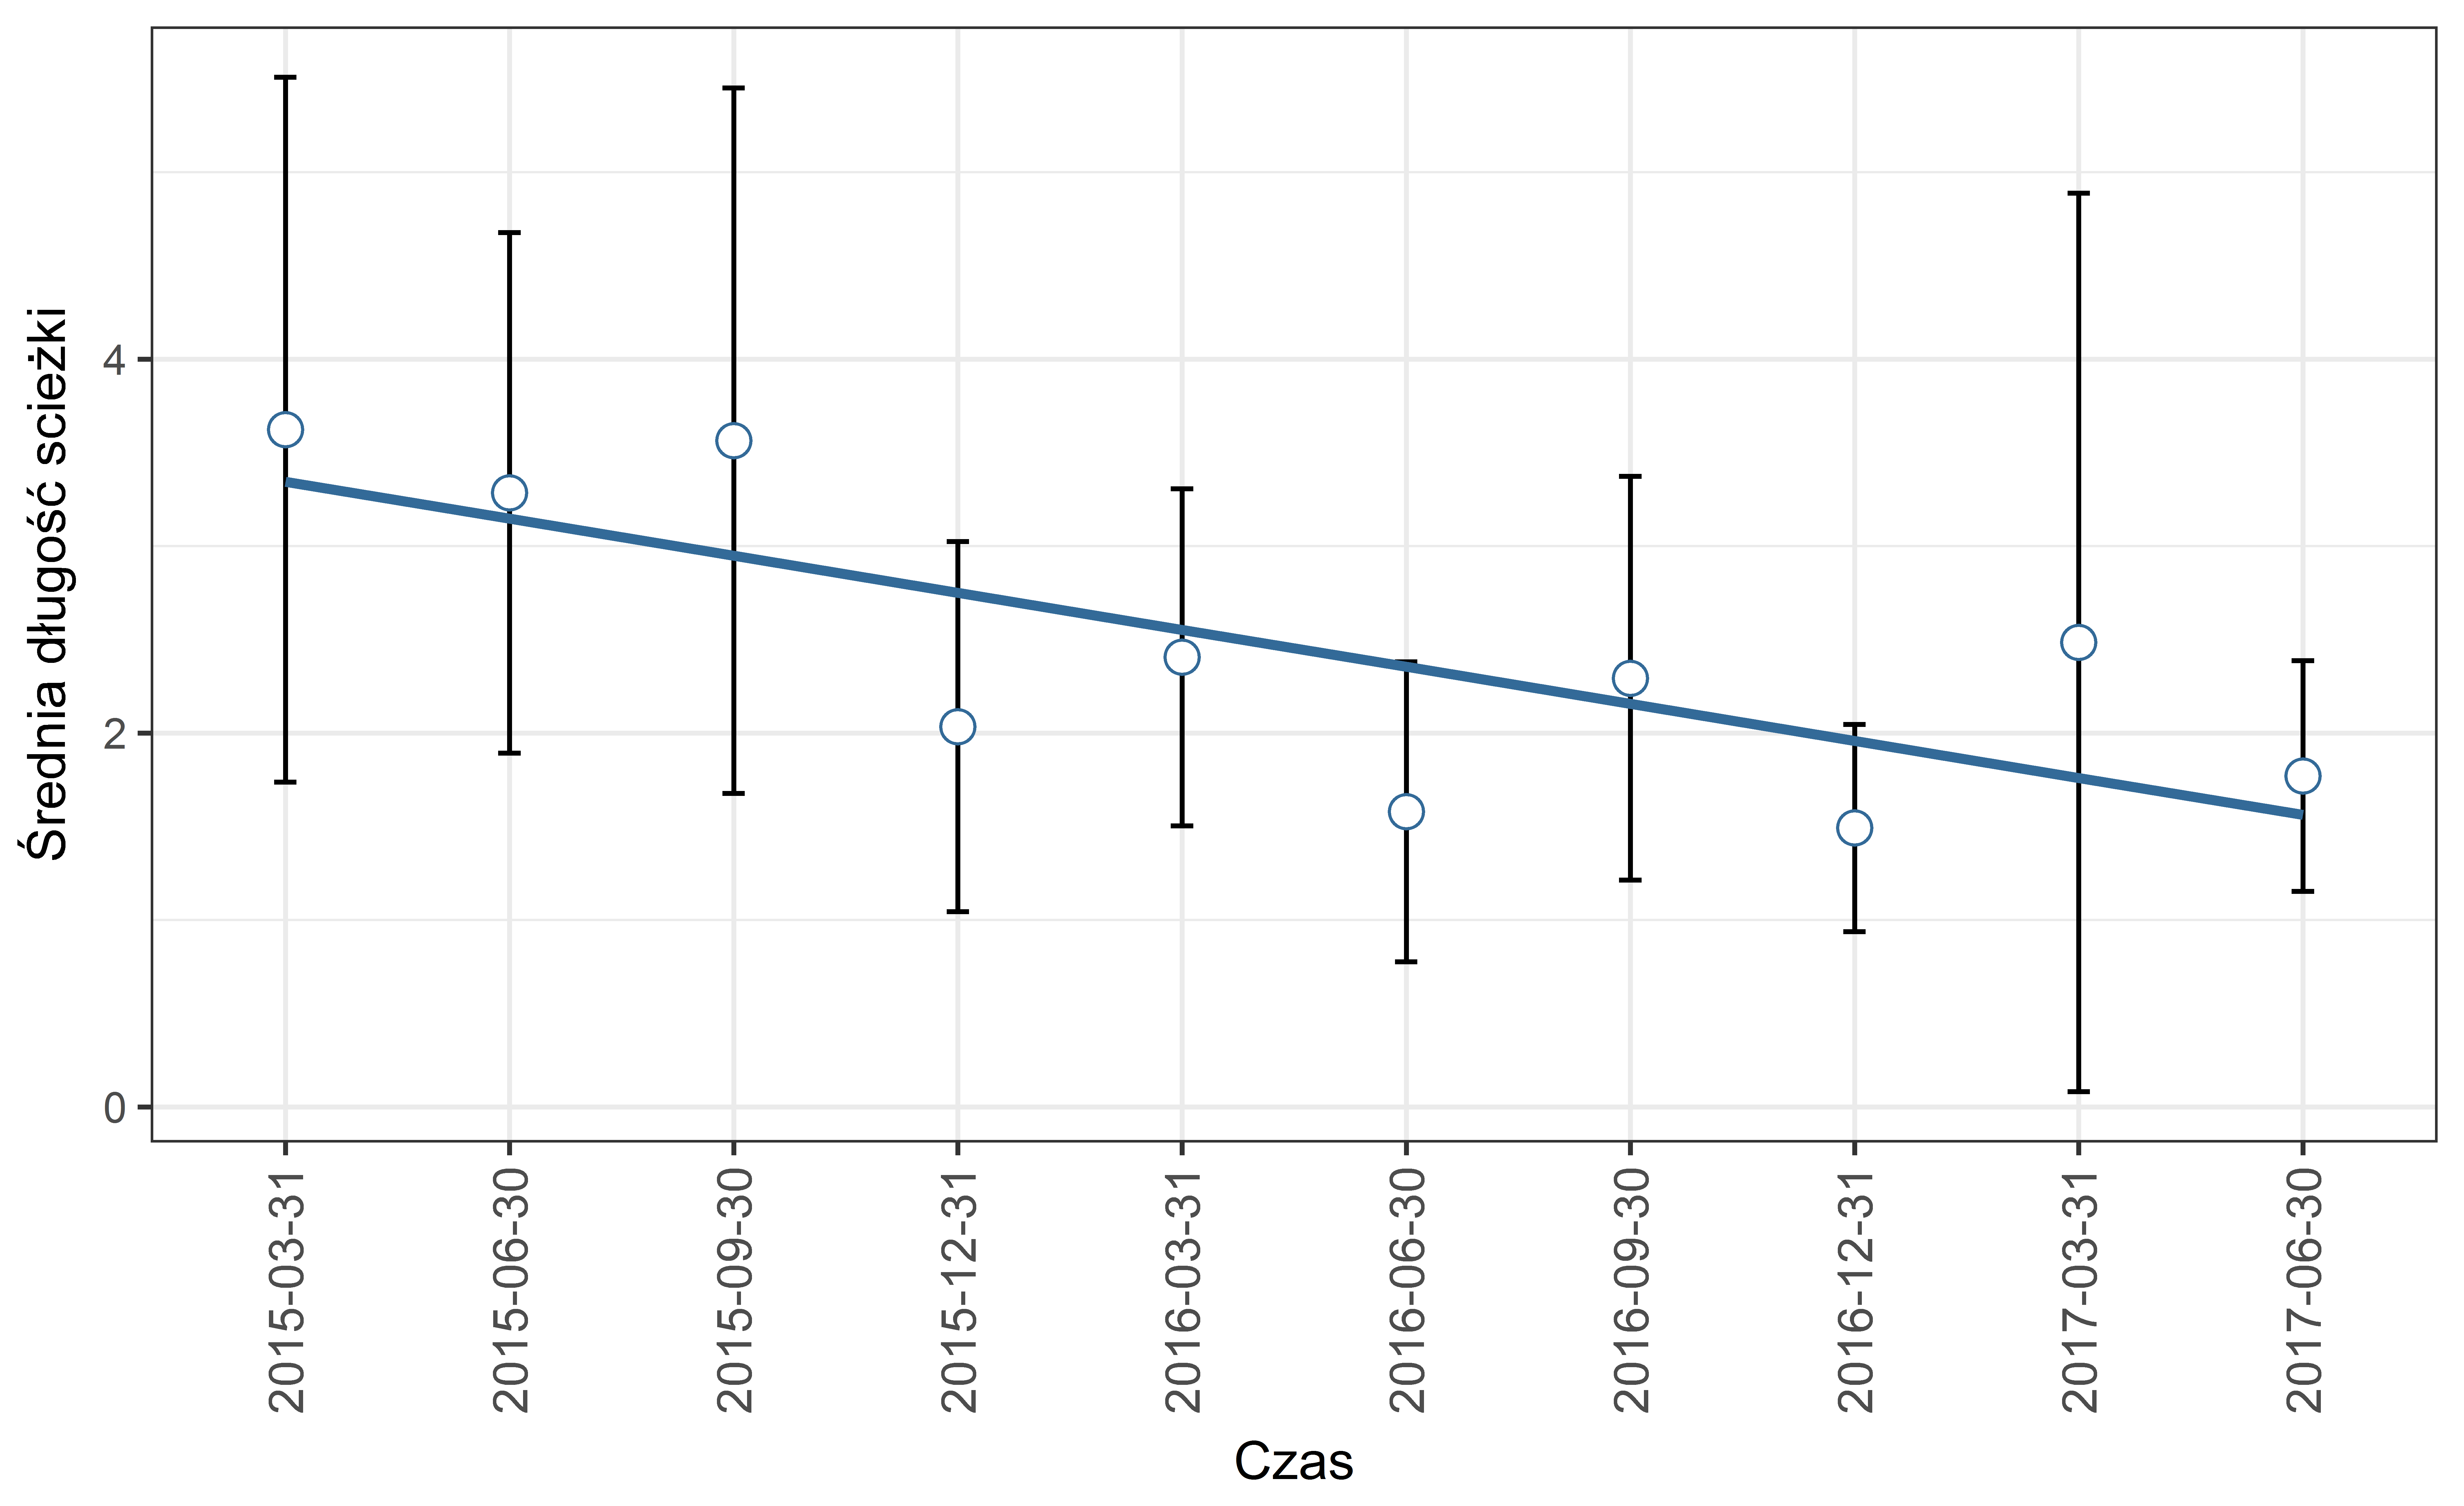
\includegraphics[width=\sizequadsda\textwidth]{pictures/srednia_dlugosc_sciezki/srednia_dlugosc_sciezki_sda.png}  \\
            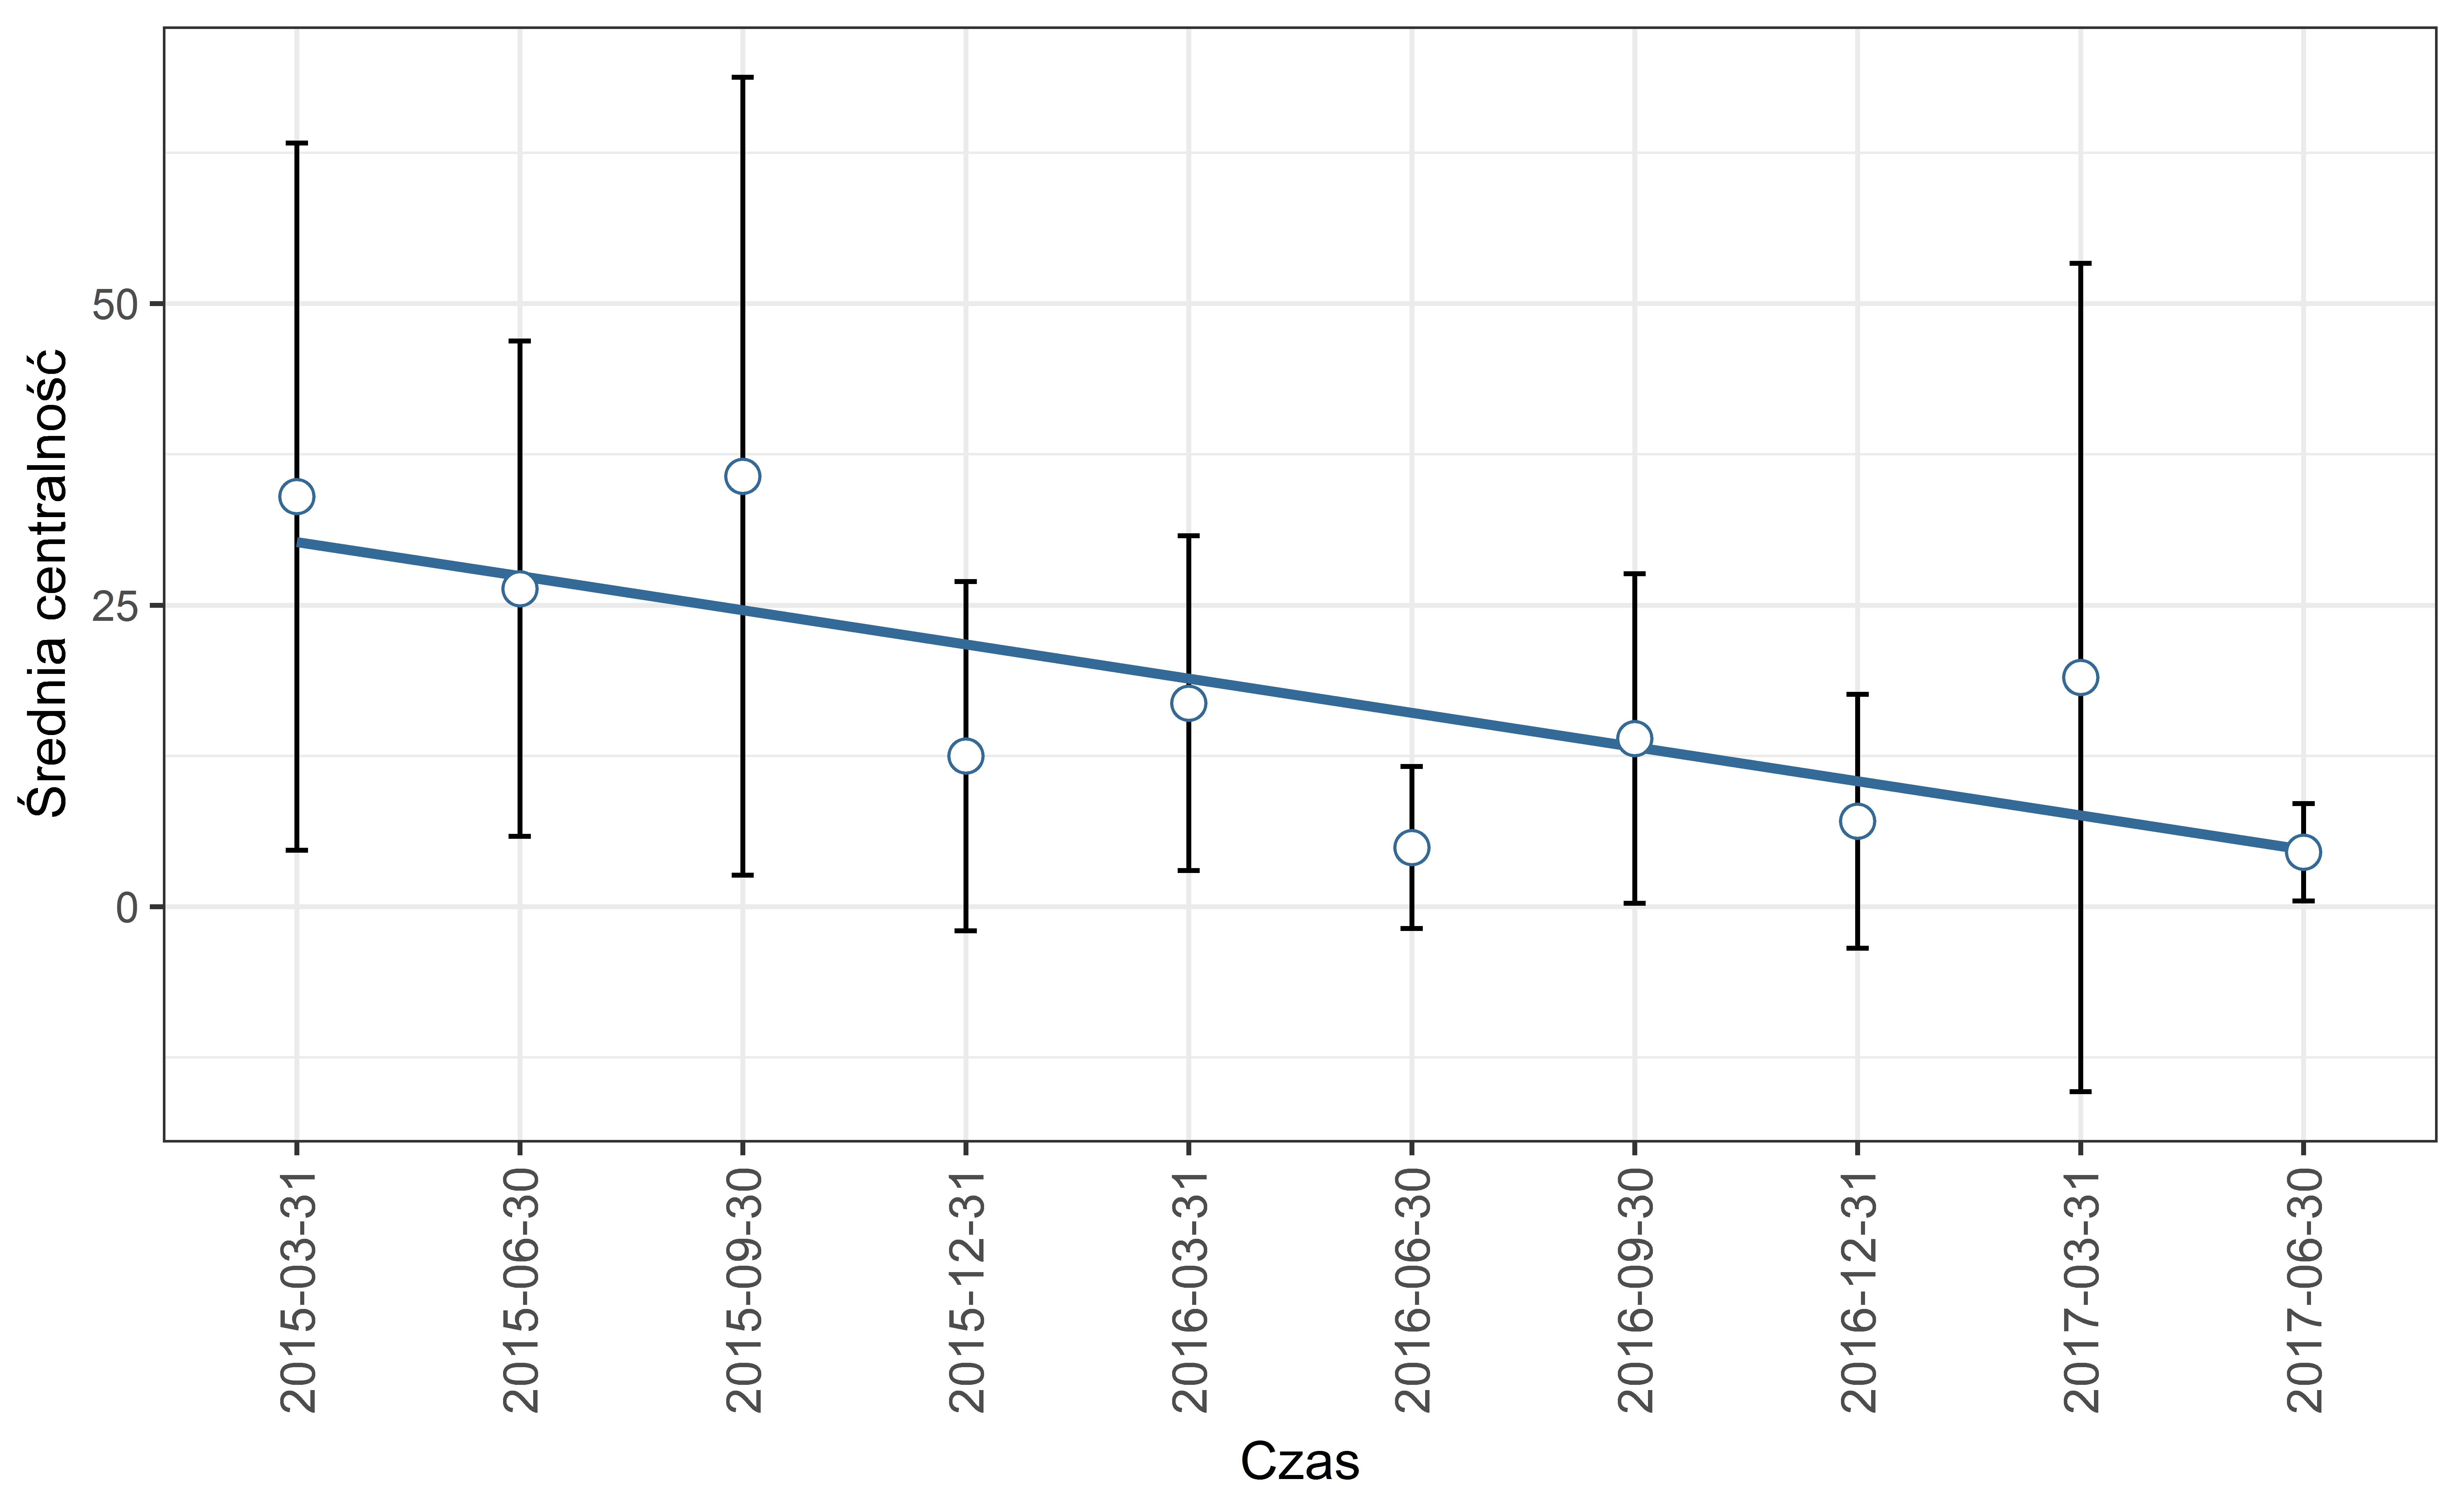
\includegraphics[width=\sizequadsda\textwidth]{pictures/srednia_centralnosc/srednia_centralnosc_sda.png}\quad
			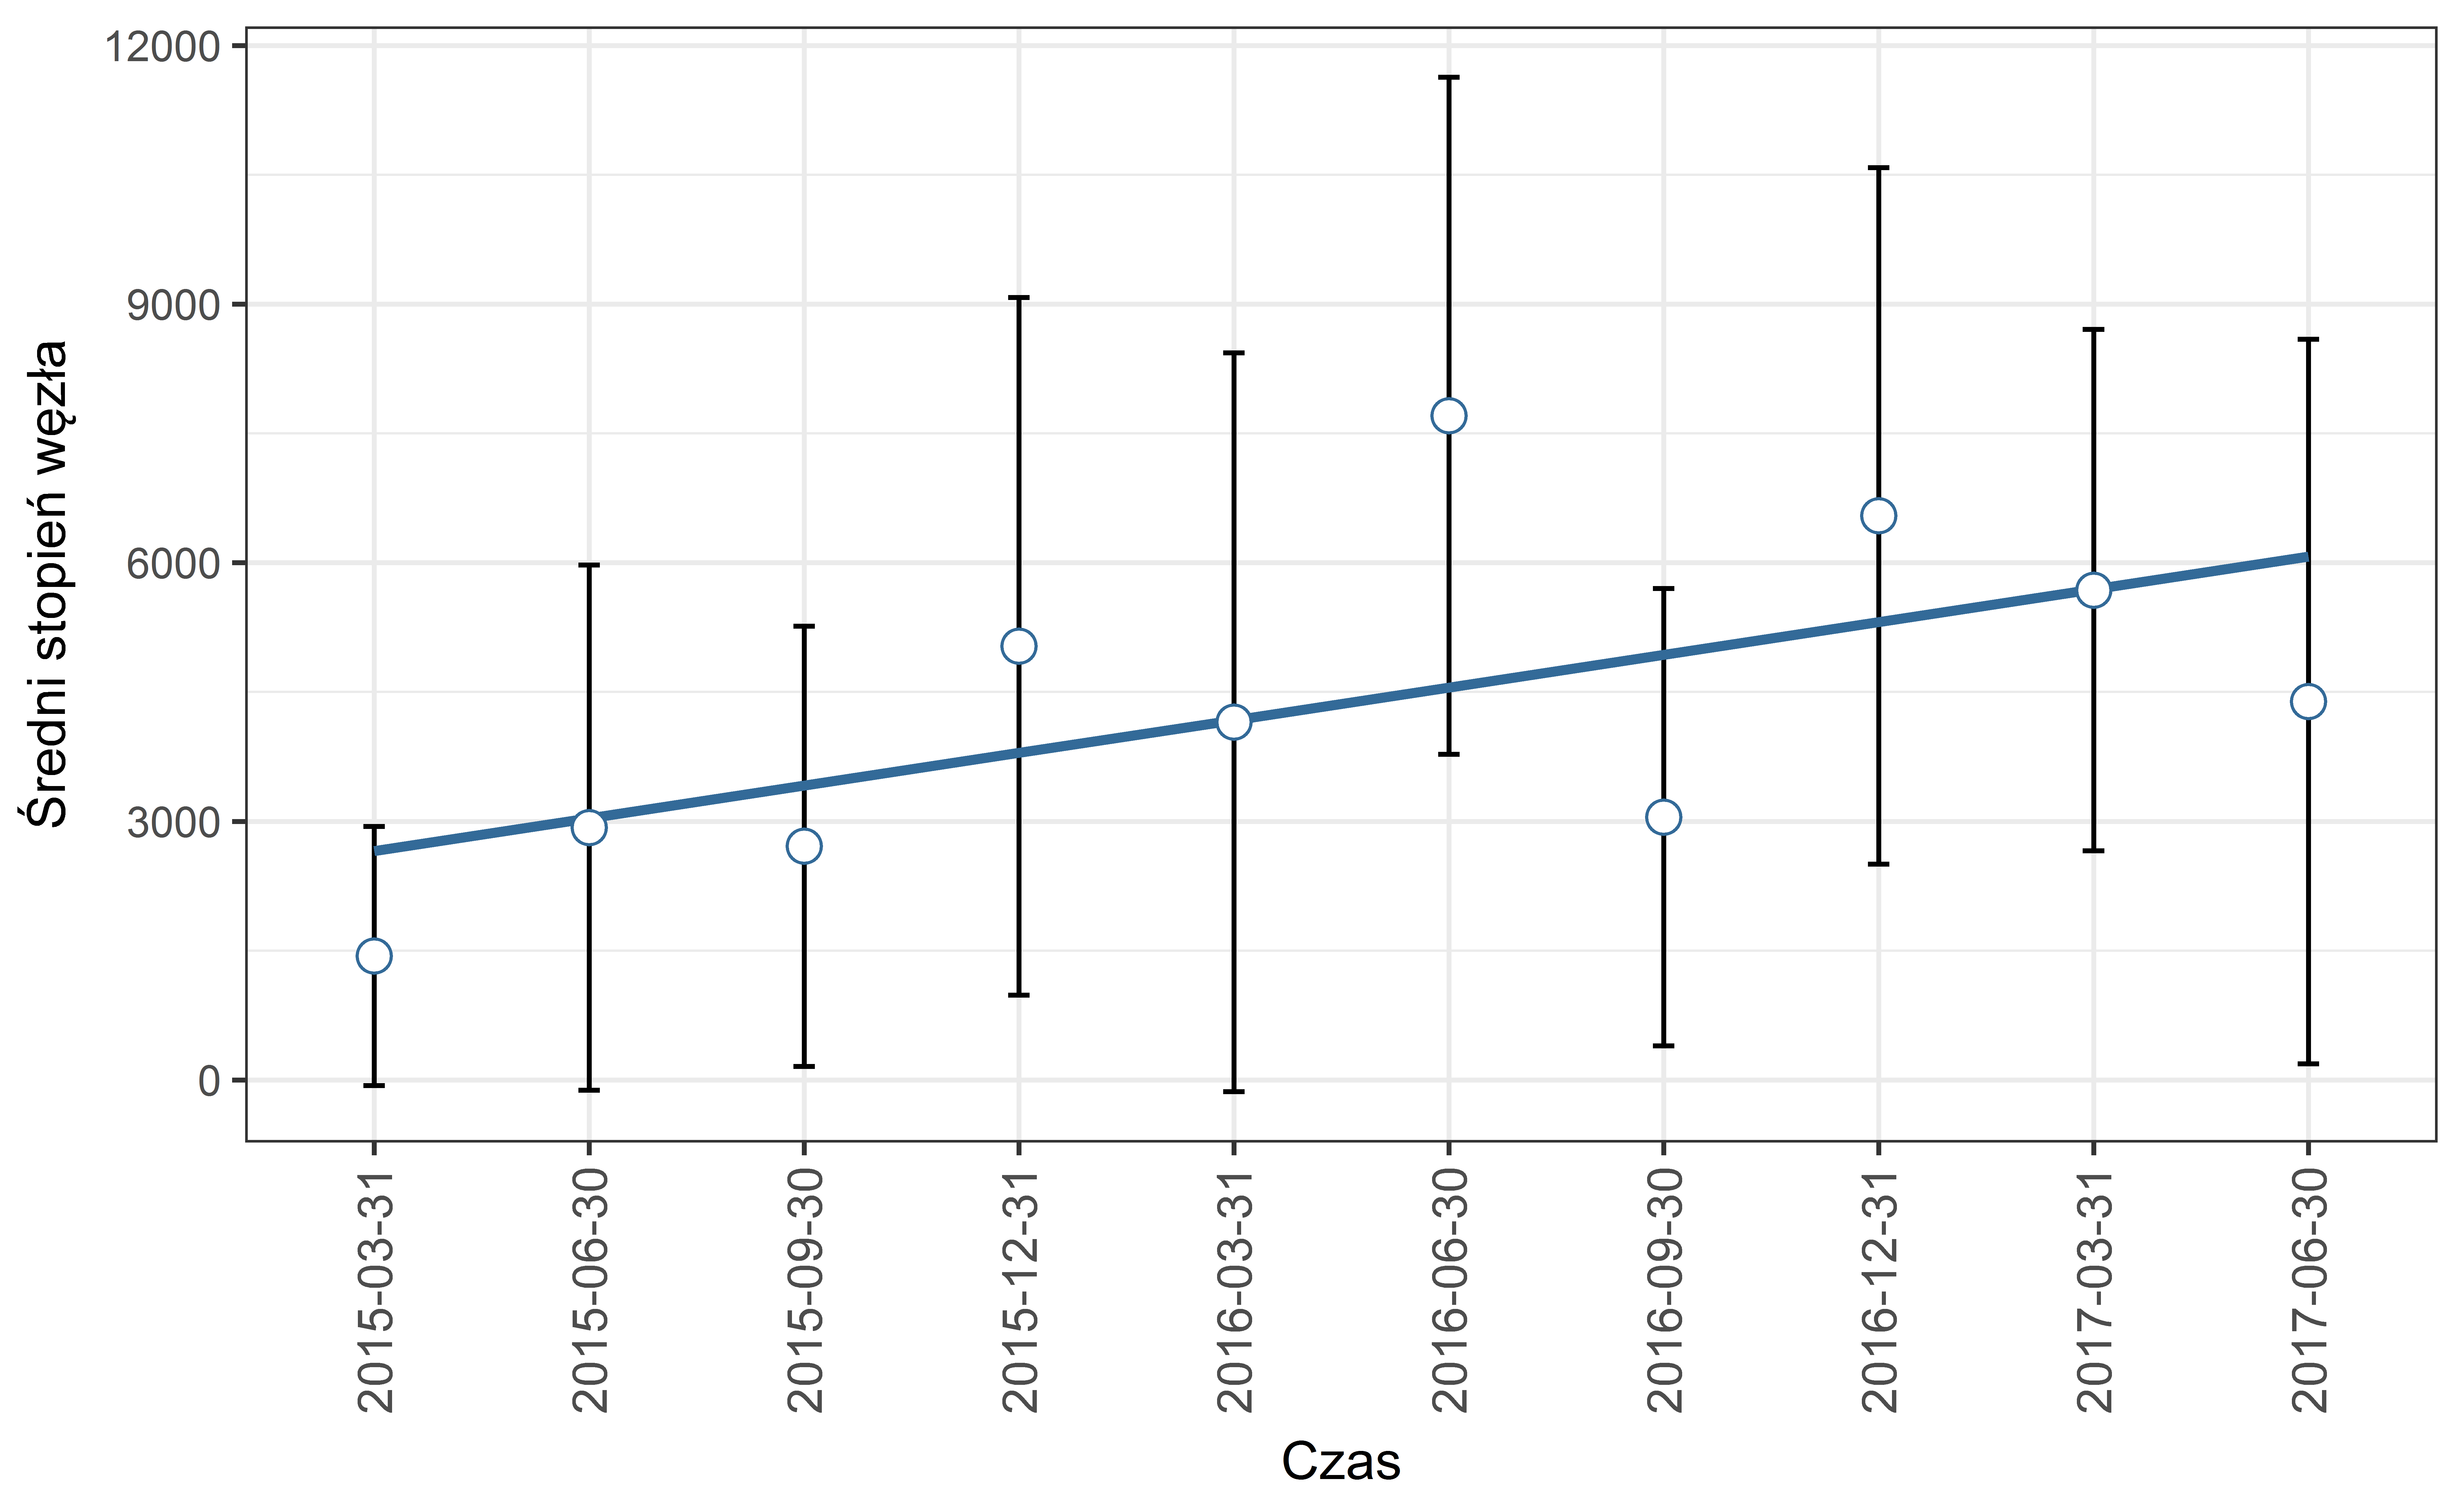
\includegraphics[width=\sizequadsda\textwidth]{pictures/sredni_stopien_wezla/sredni_stopien_wezla_sda.png}
 \end{minipage} 
\end{frame}

\begin{frame}
 \frametitle{Wyniki}
 \framesubtitle{Własności sieci wynikające z jej specyfiki}
   \begin{minipage}{\textwidth}
     \centering
 		  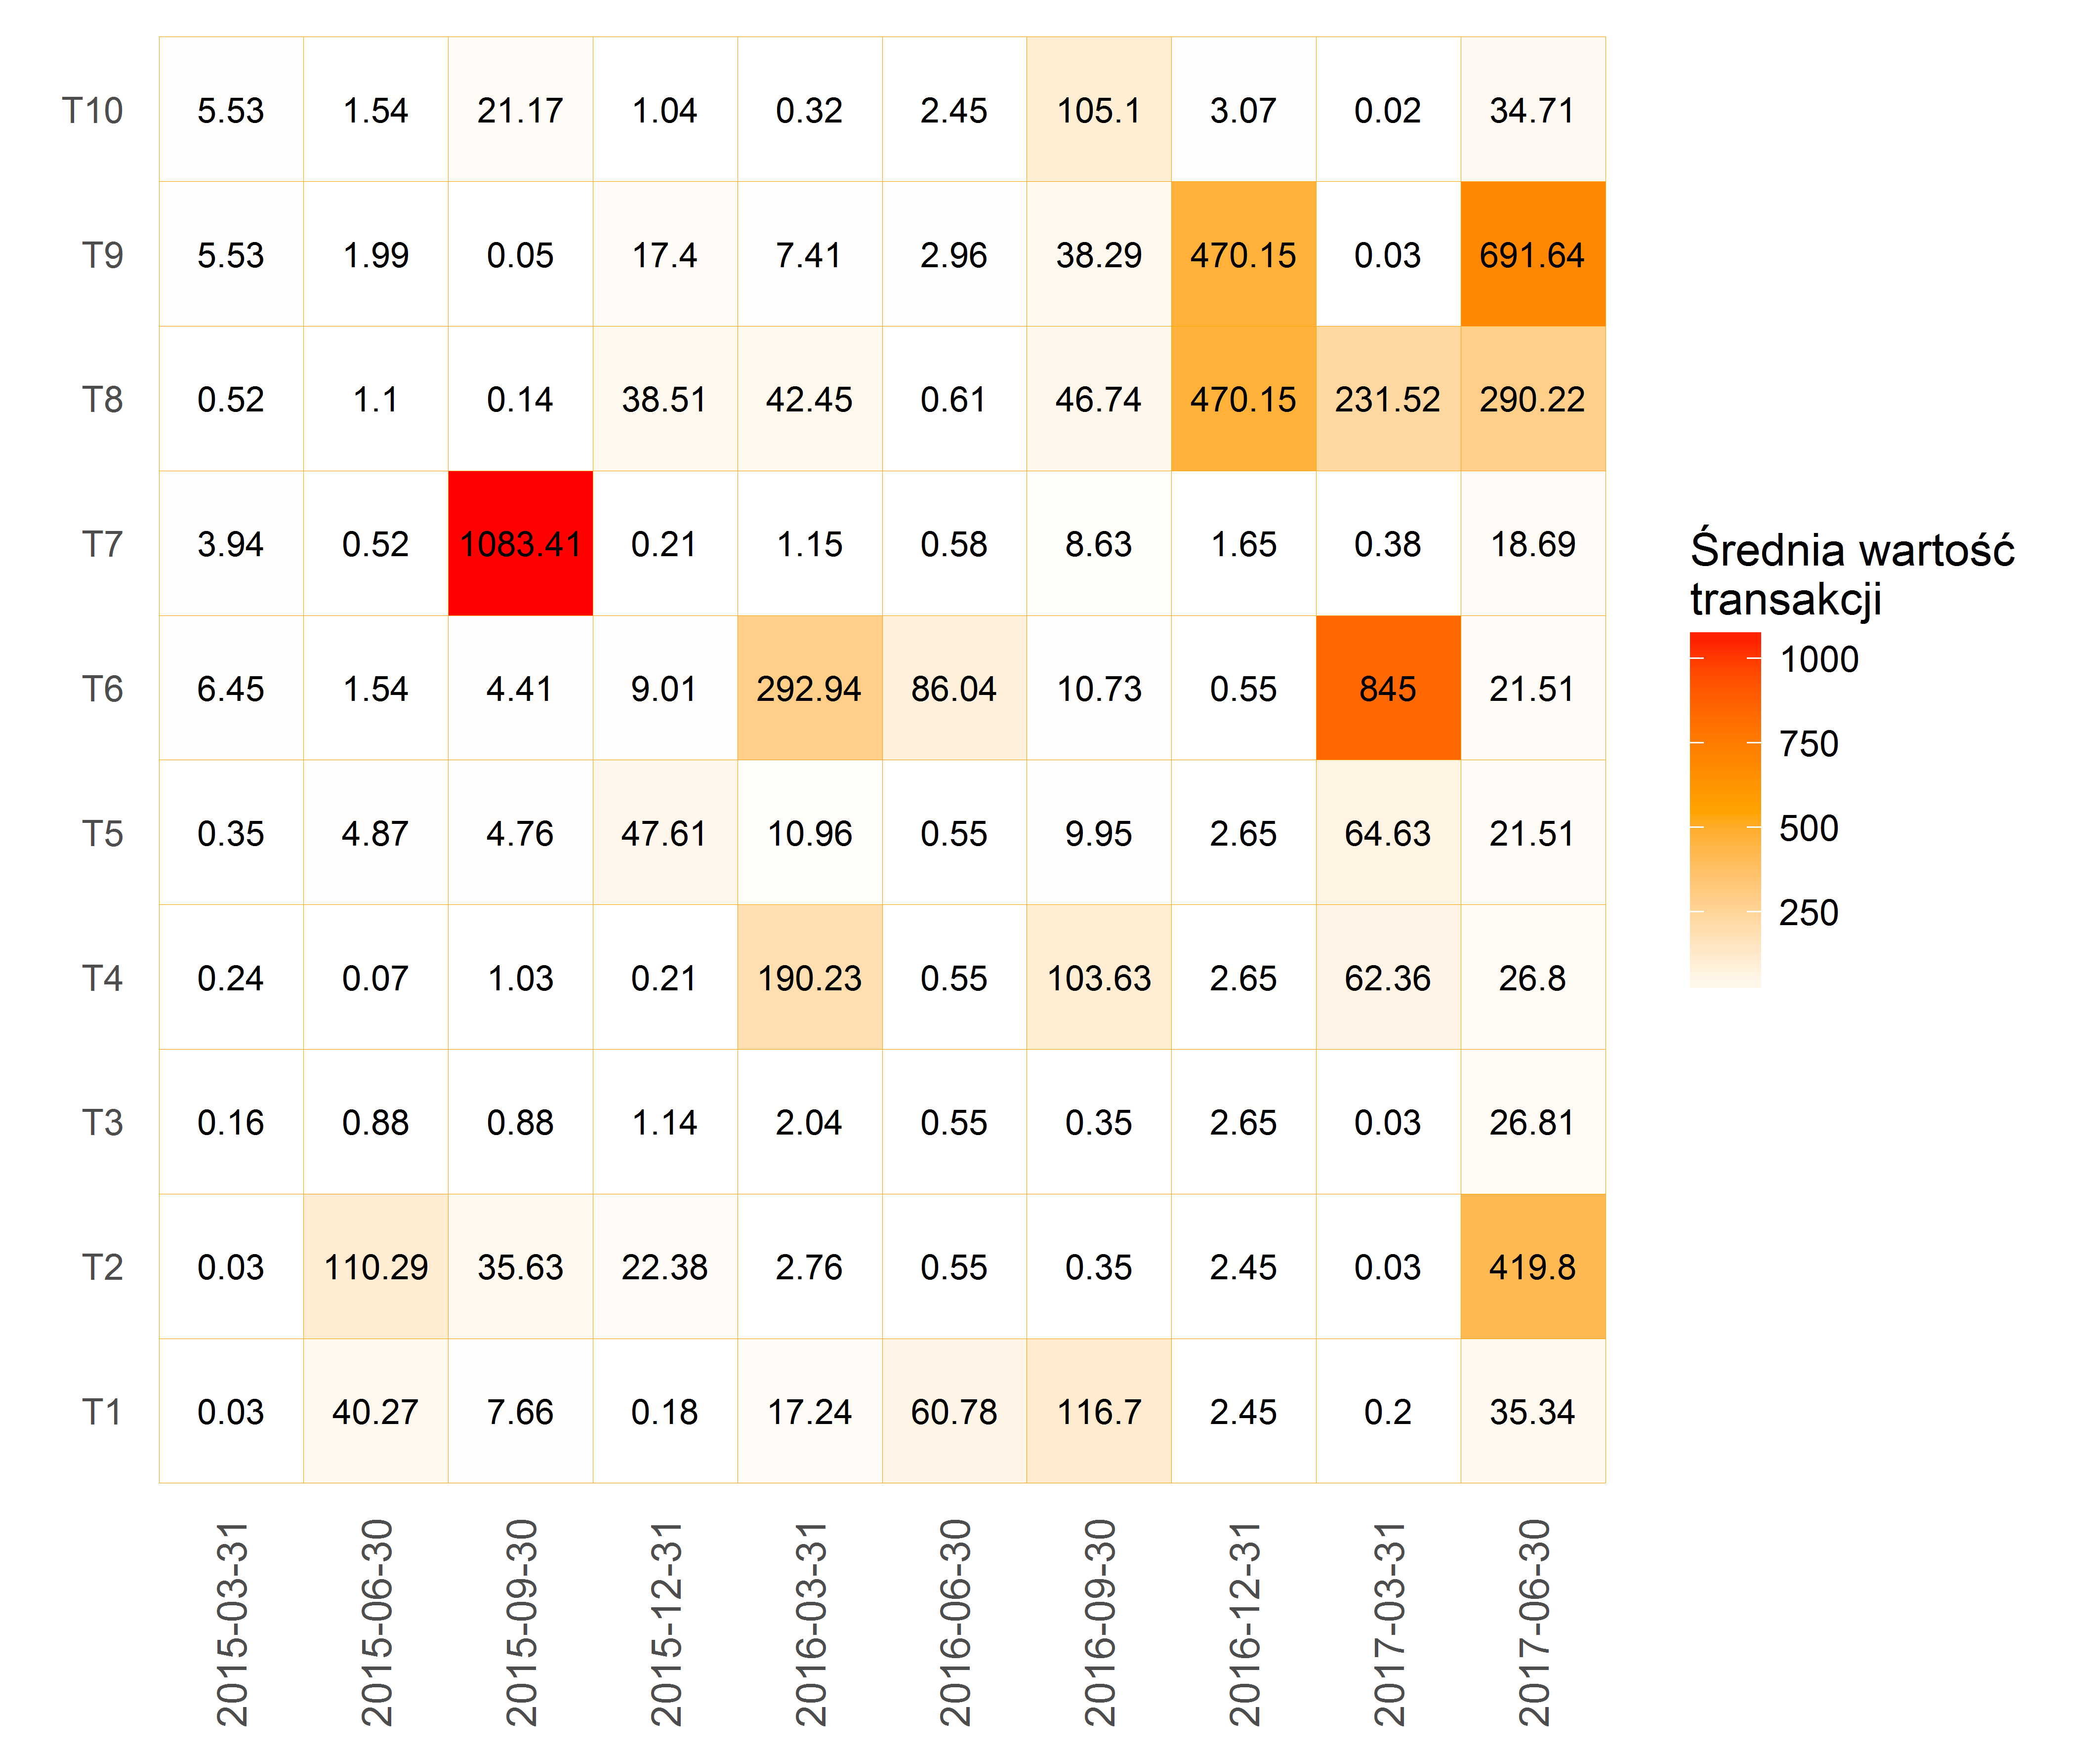
\includegraphics[width=\sizequad\textwidth]{pictures/wartosc_transakcji/wartosc_transakcji_hm.png}\quad  
  		 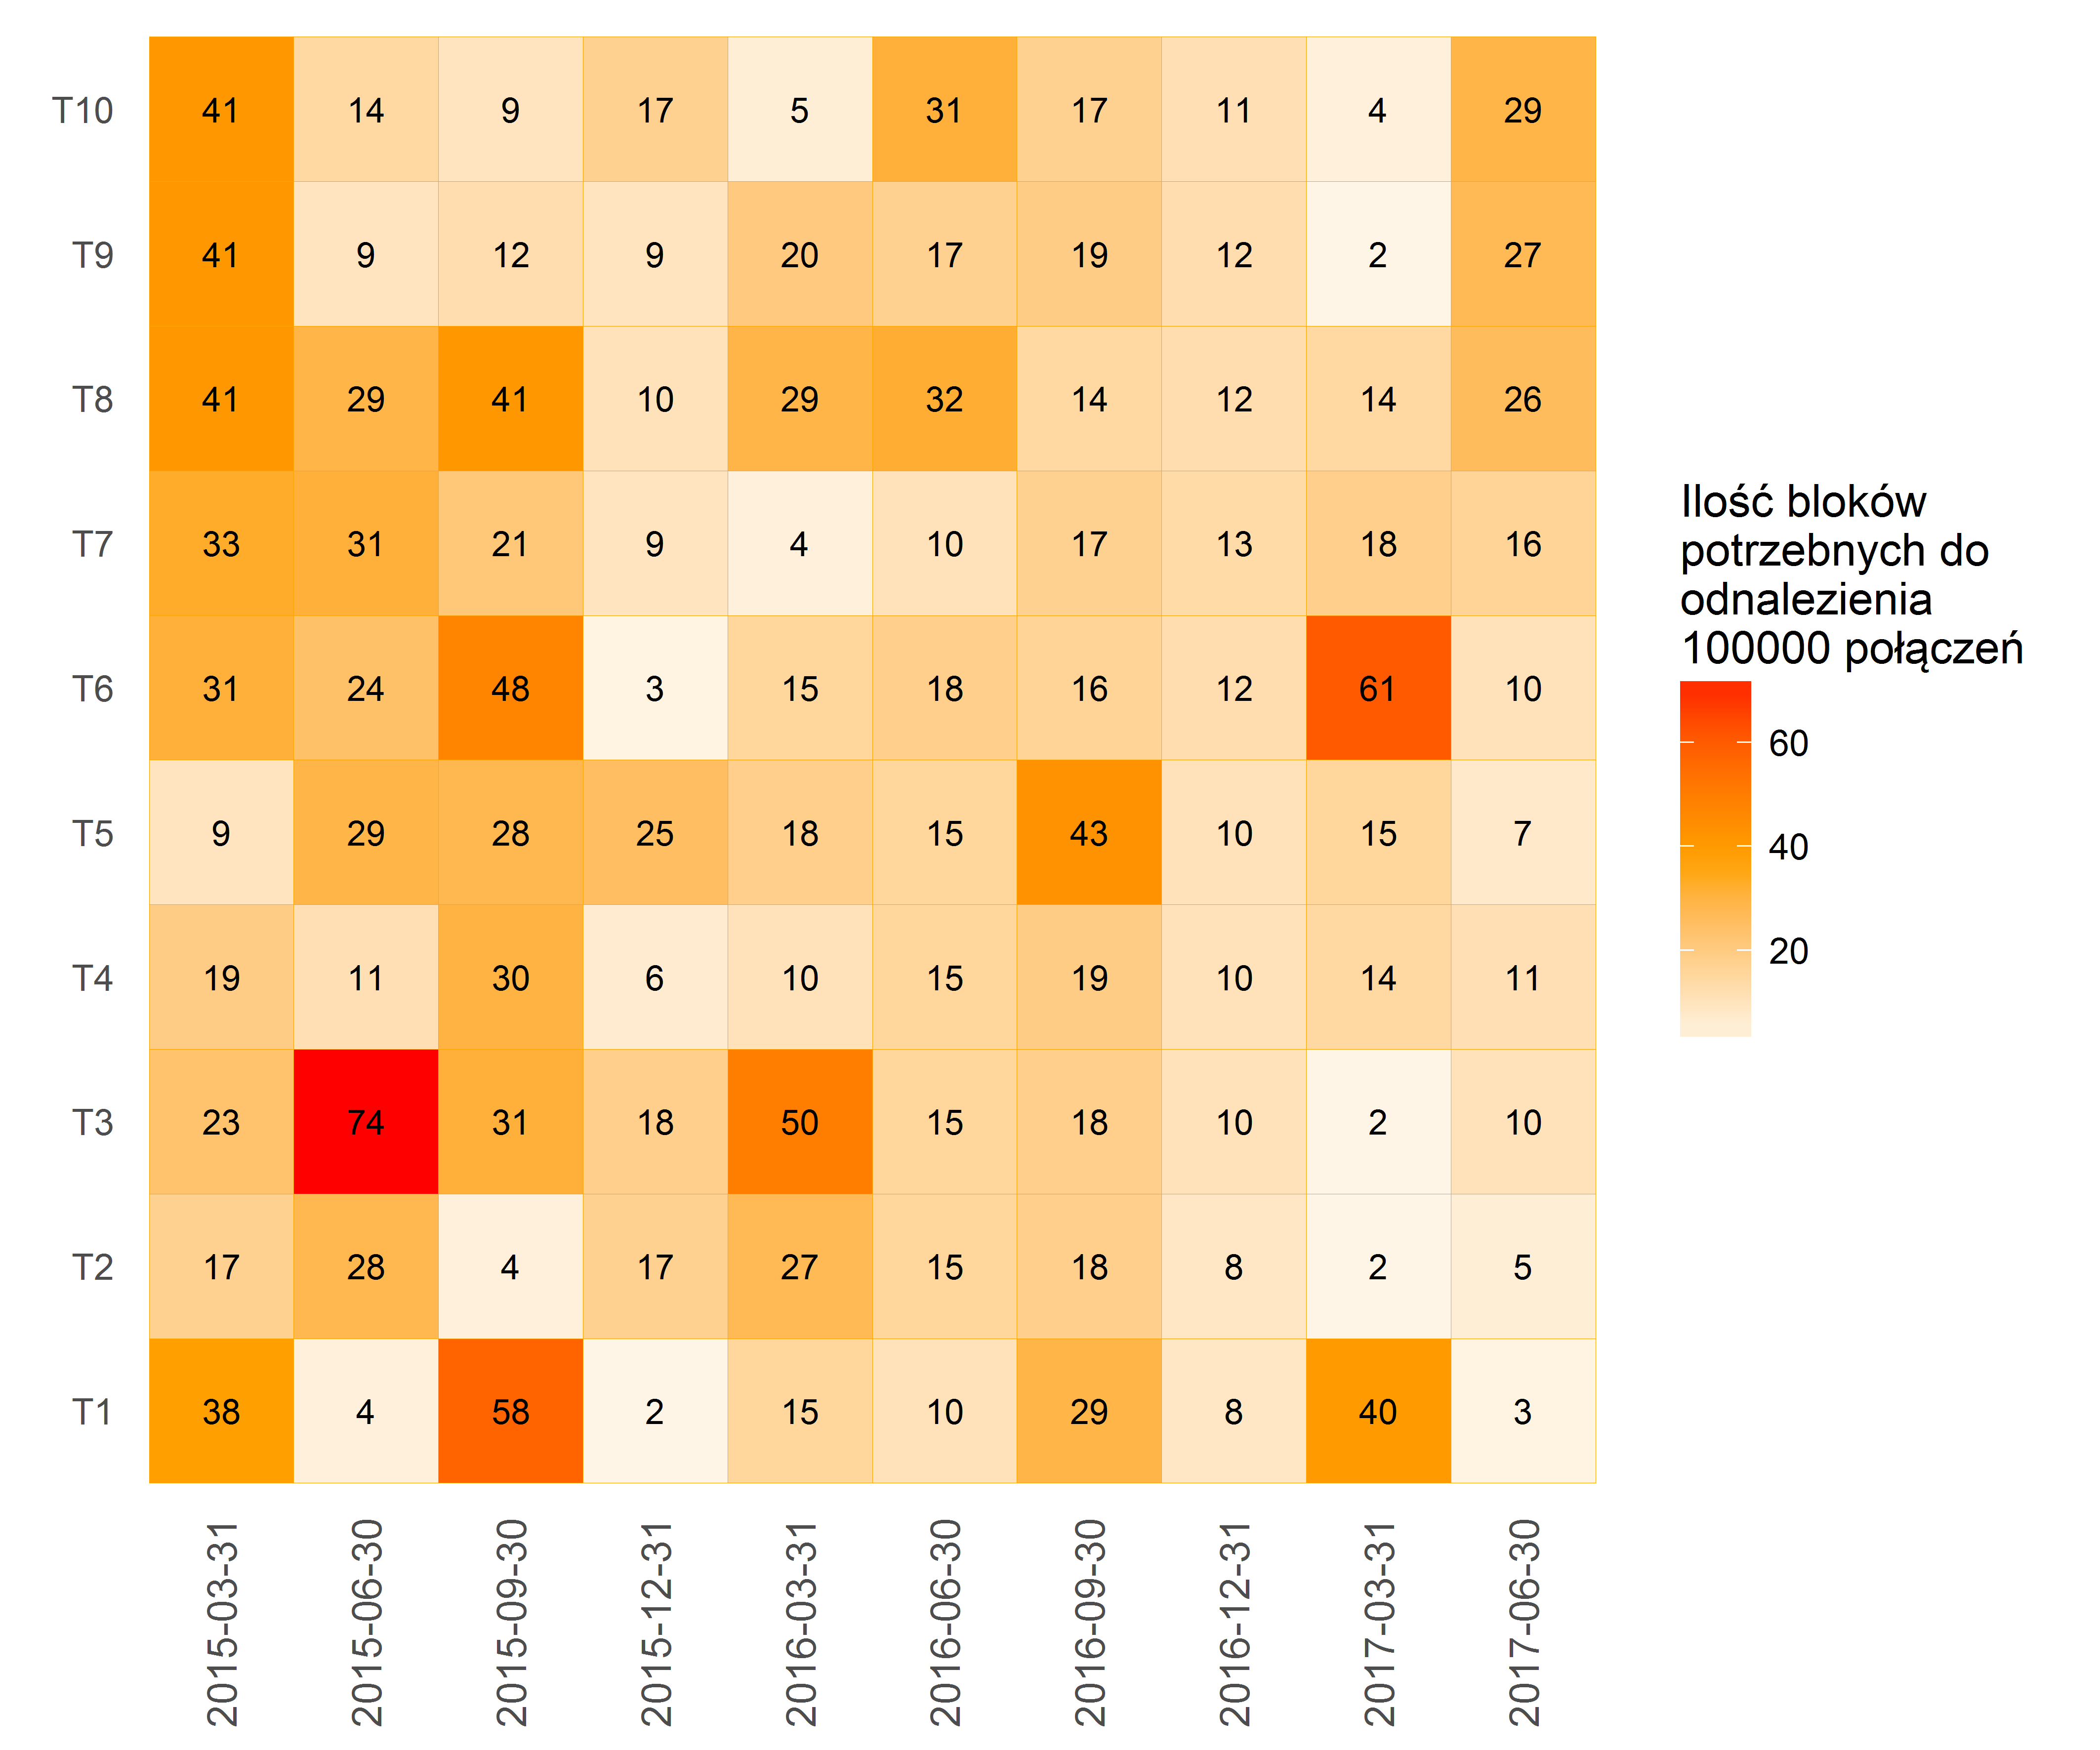
\includegraphics[width=\sizequad\textwidth]{pictures/ilosc_blokow/ilosc_blokow_hm.png}  \\
  		 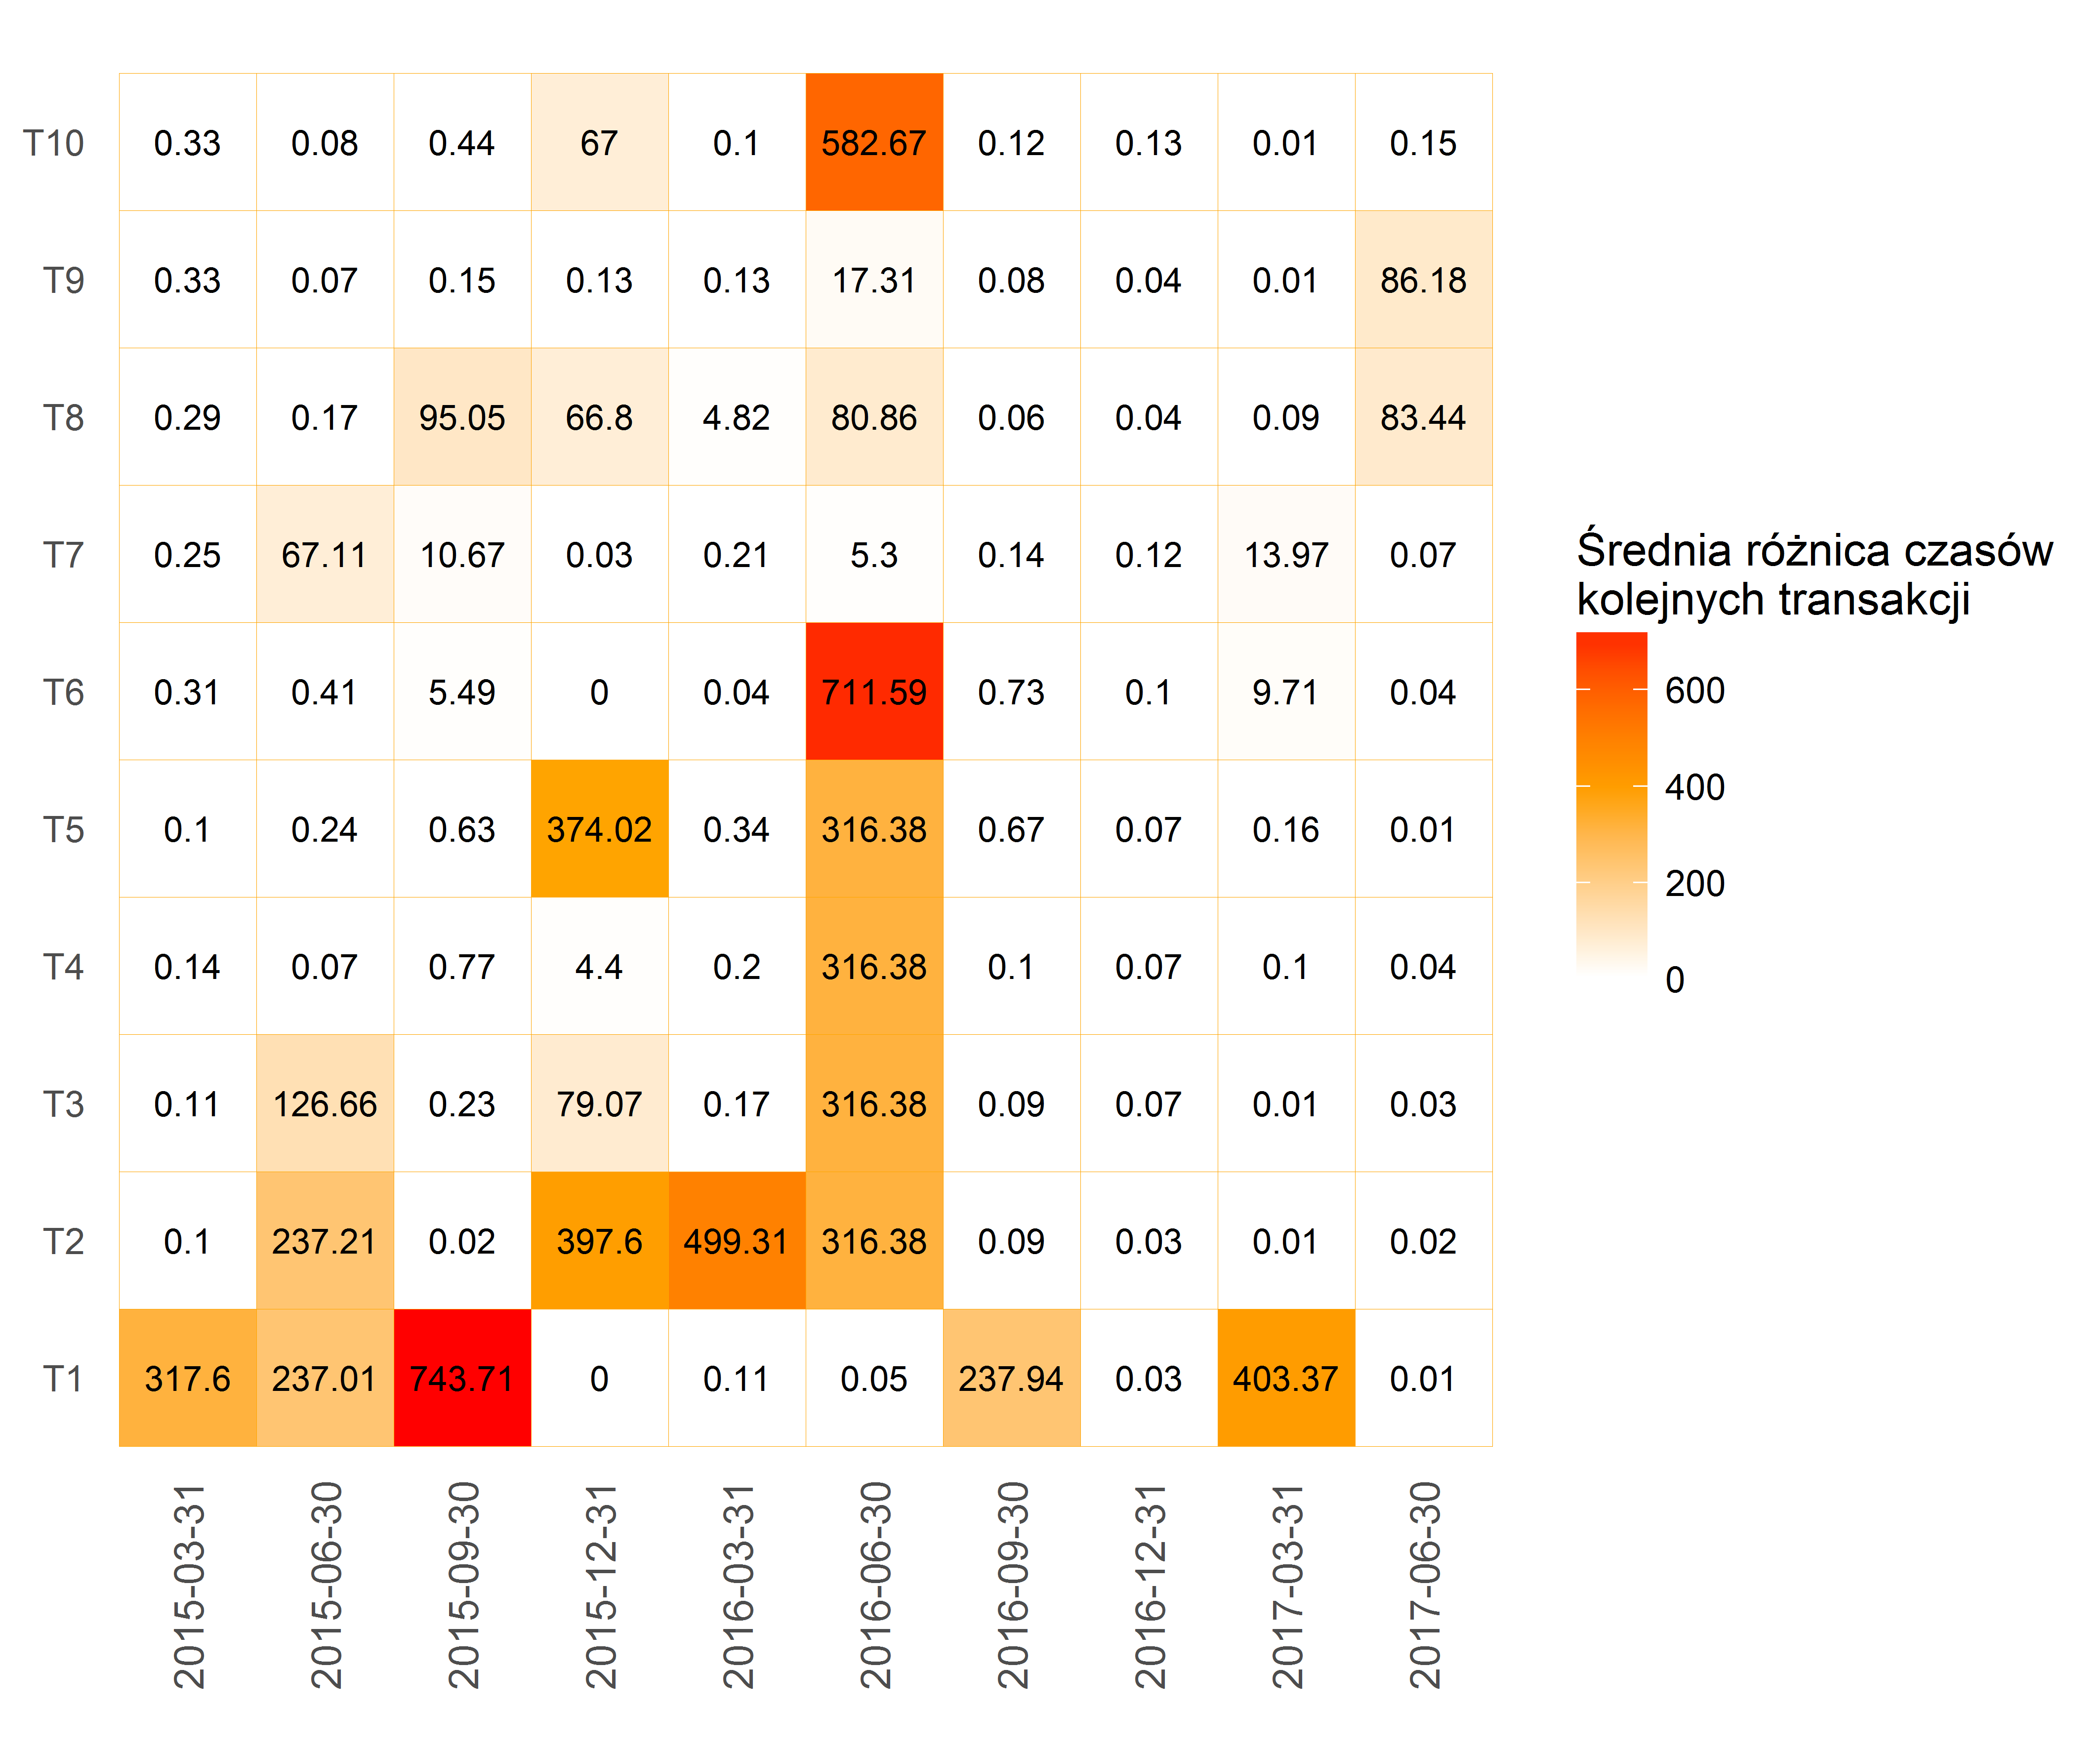
\includegraphics[width=\sizequad\textwidth]{pictures/roznica_czasow/roznica_czasow_hm.png}\quad
  		 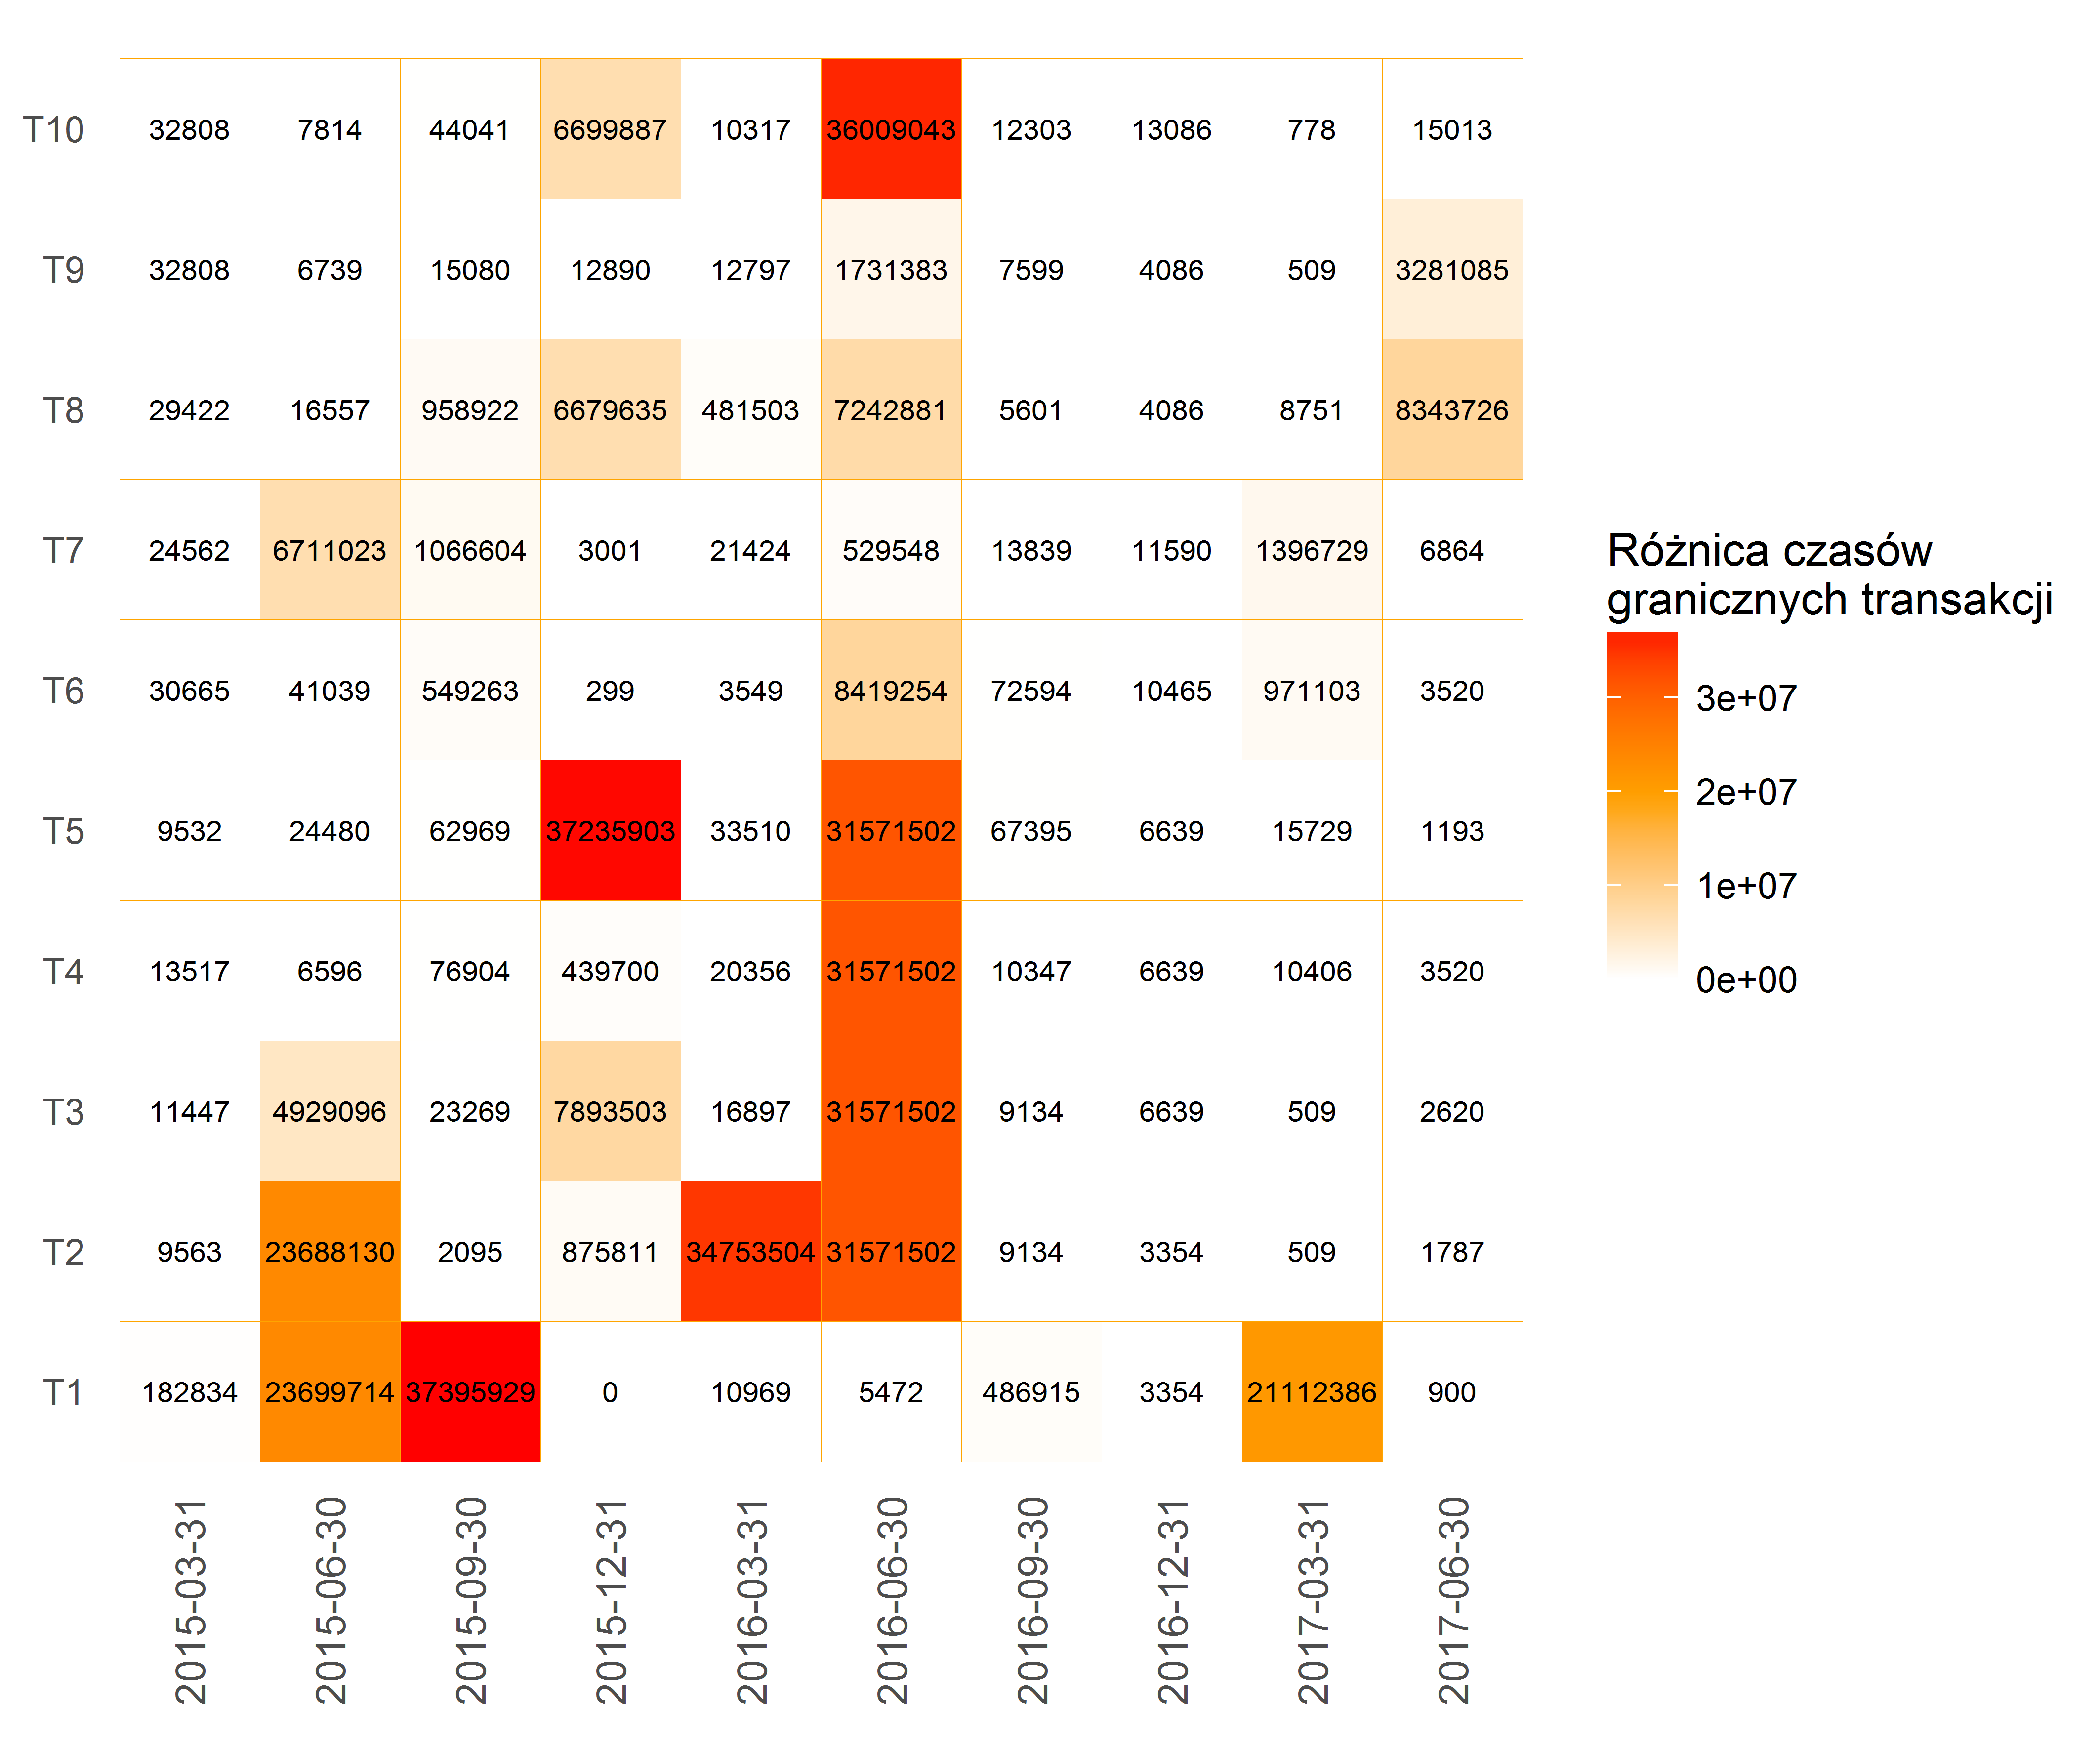
\includegraphics[width=\sizequad\textwidth]{pictures/czas_graniczny/czas_graniczny_hm.png}
 \end{minipage} 
\end{frame}

\begin{frame}
 \frametitle{Trend}
 \framesubtitle{Własności sieci wynikające z jej specyfiki}
    \begin{minipage}{\textwidth}
 		  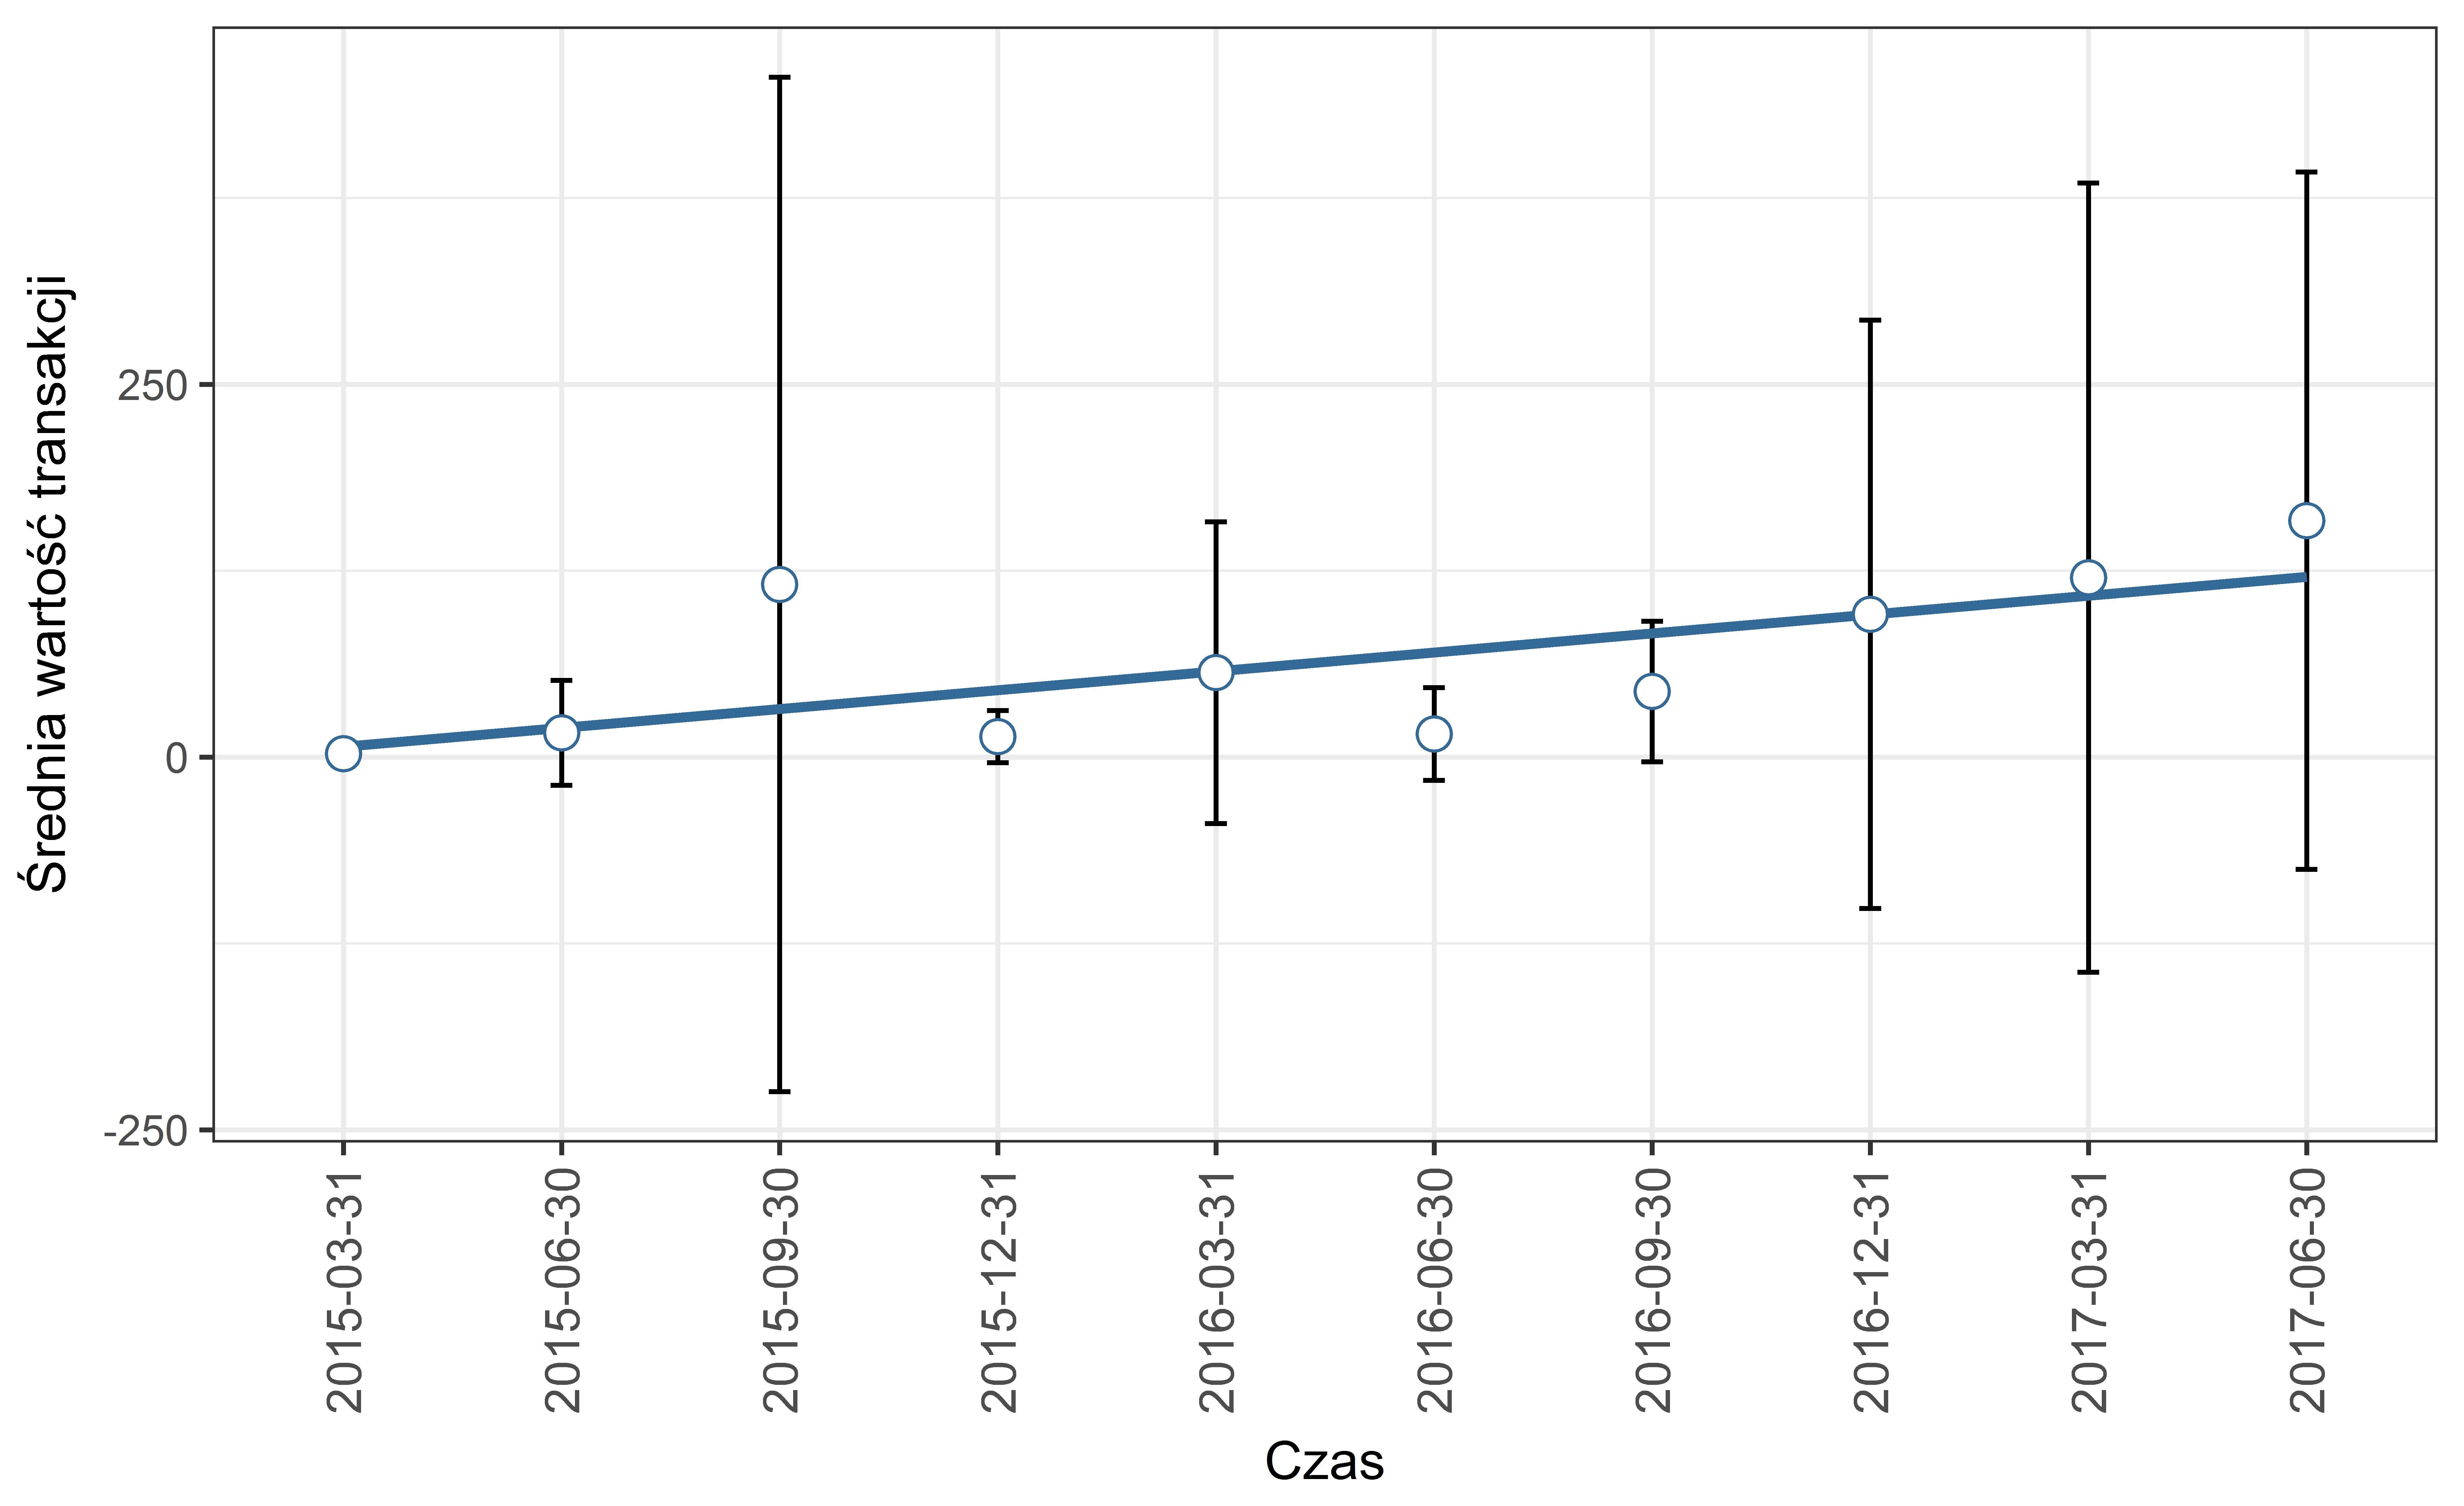
\includegraphics[width=\sizequadsda\textwidth]{pictures/wartosc_transakcji/wartosc_transakcji_sda.png}\quad  
  		 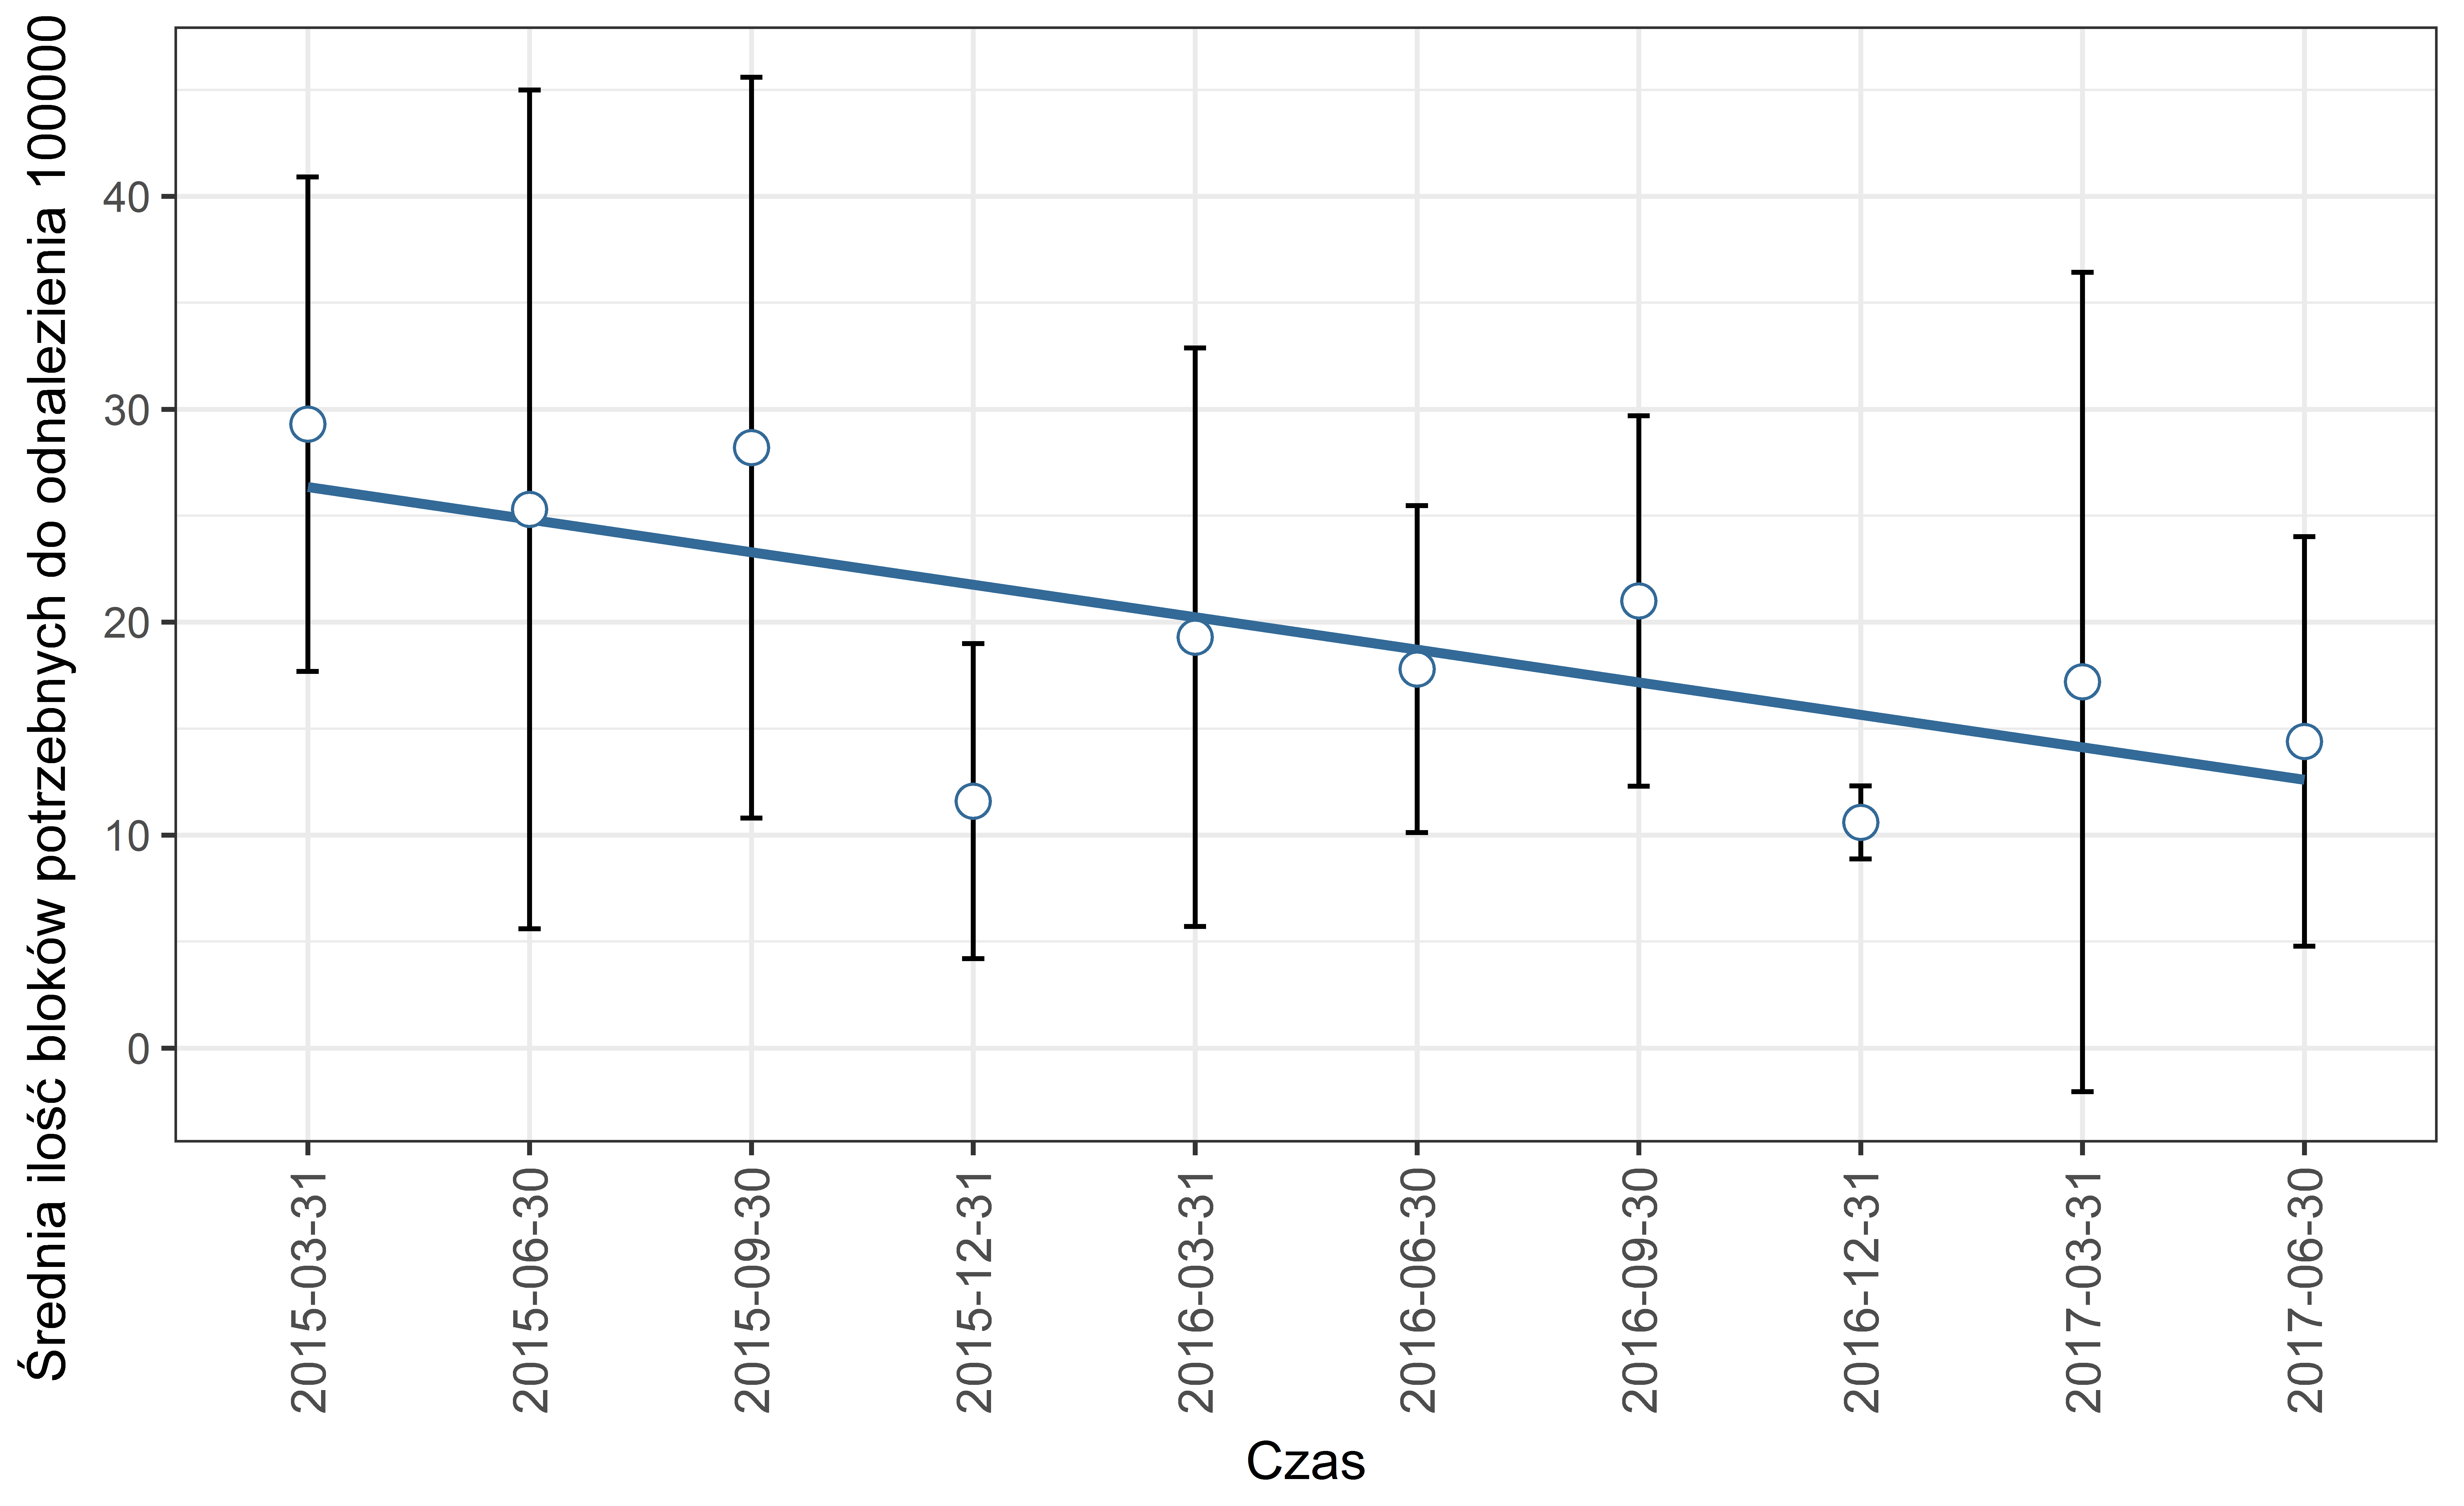
\includegraphics[width=\sizequadsda\textwidth]{pictures/ilosc_blokow/ilosc_blokow_sda.png}  \\
  		 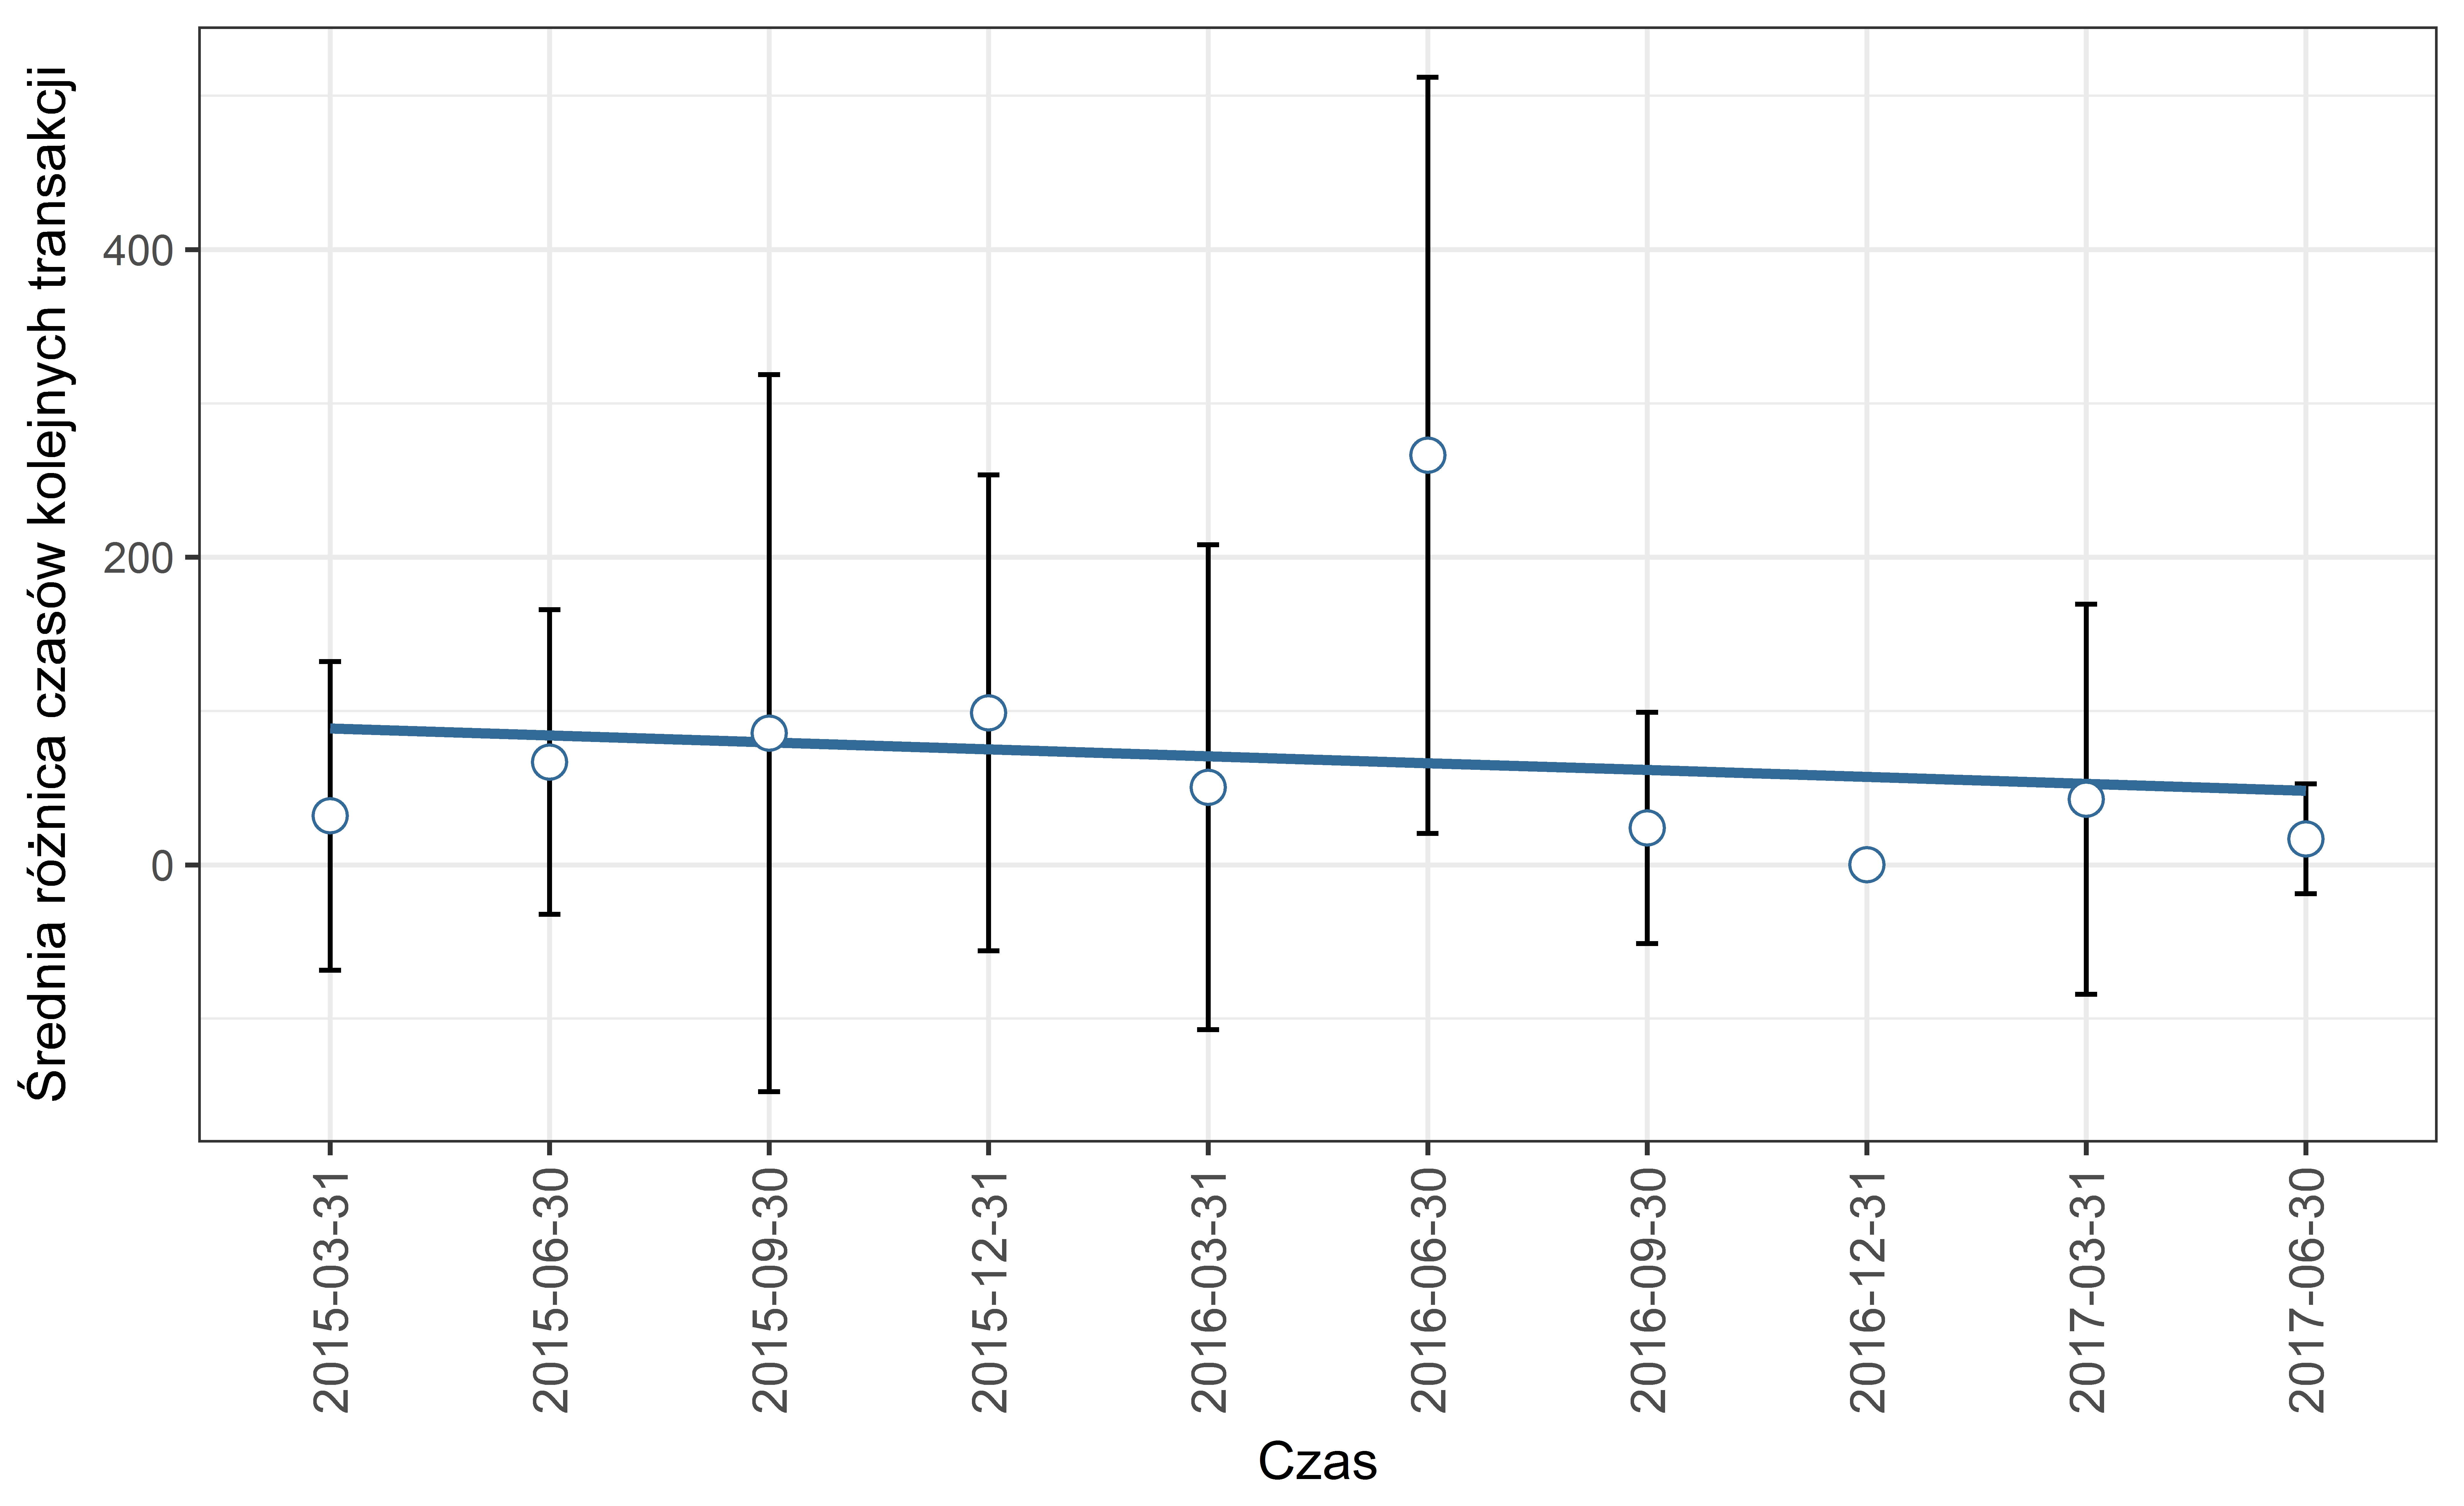
\includegraphics[width=\sizequadsda\textwidth]{pictures/roznica_czasow/roznica_czasow_sda.png}\quad
  		 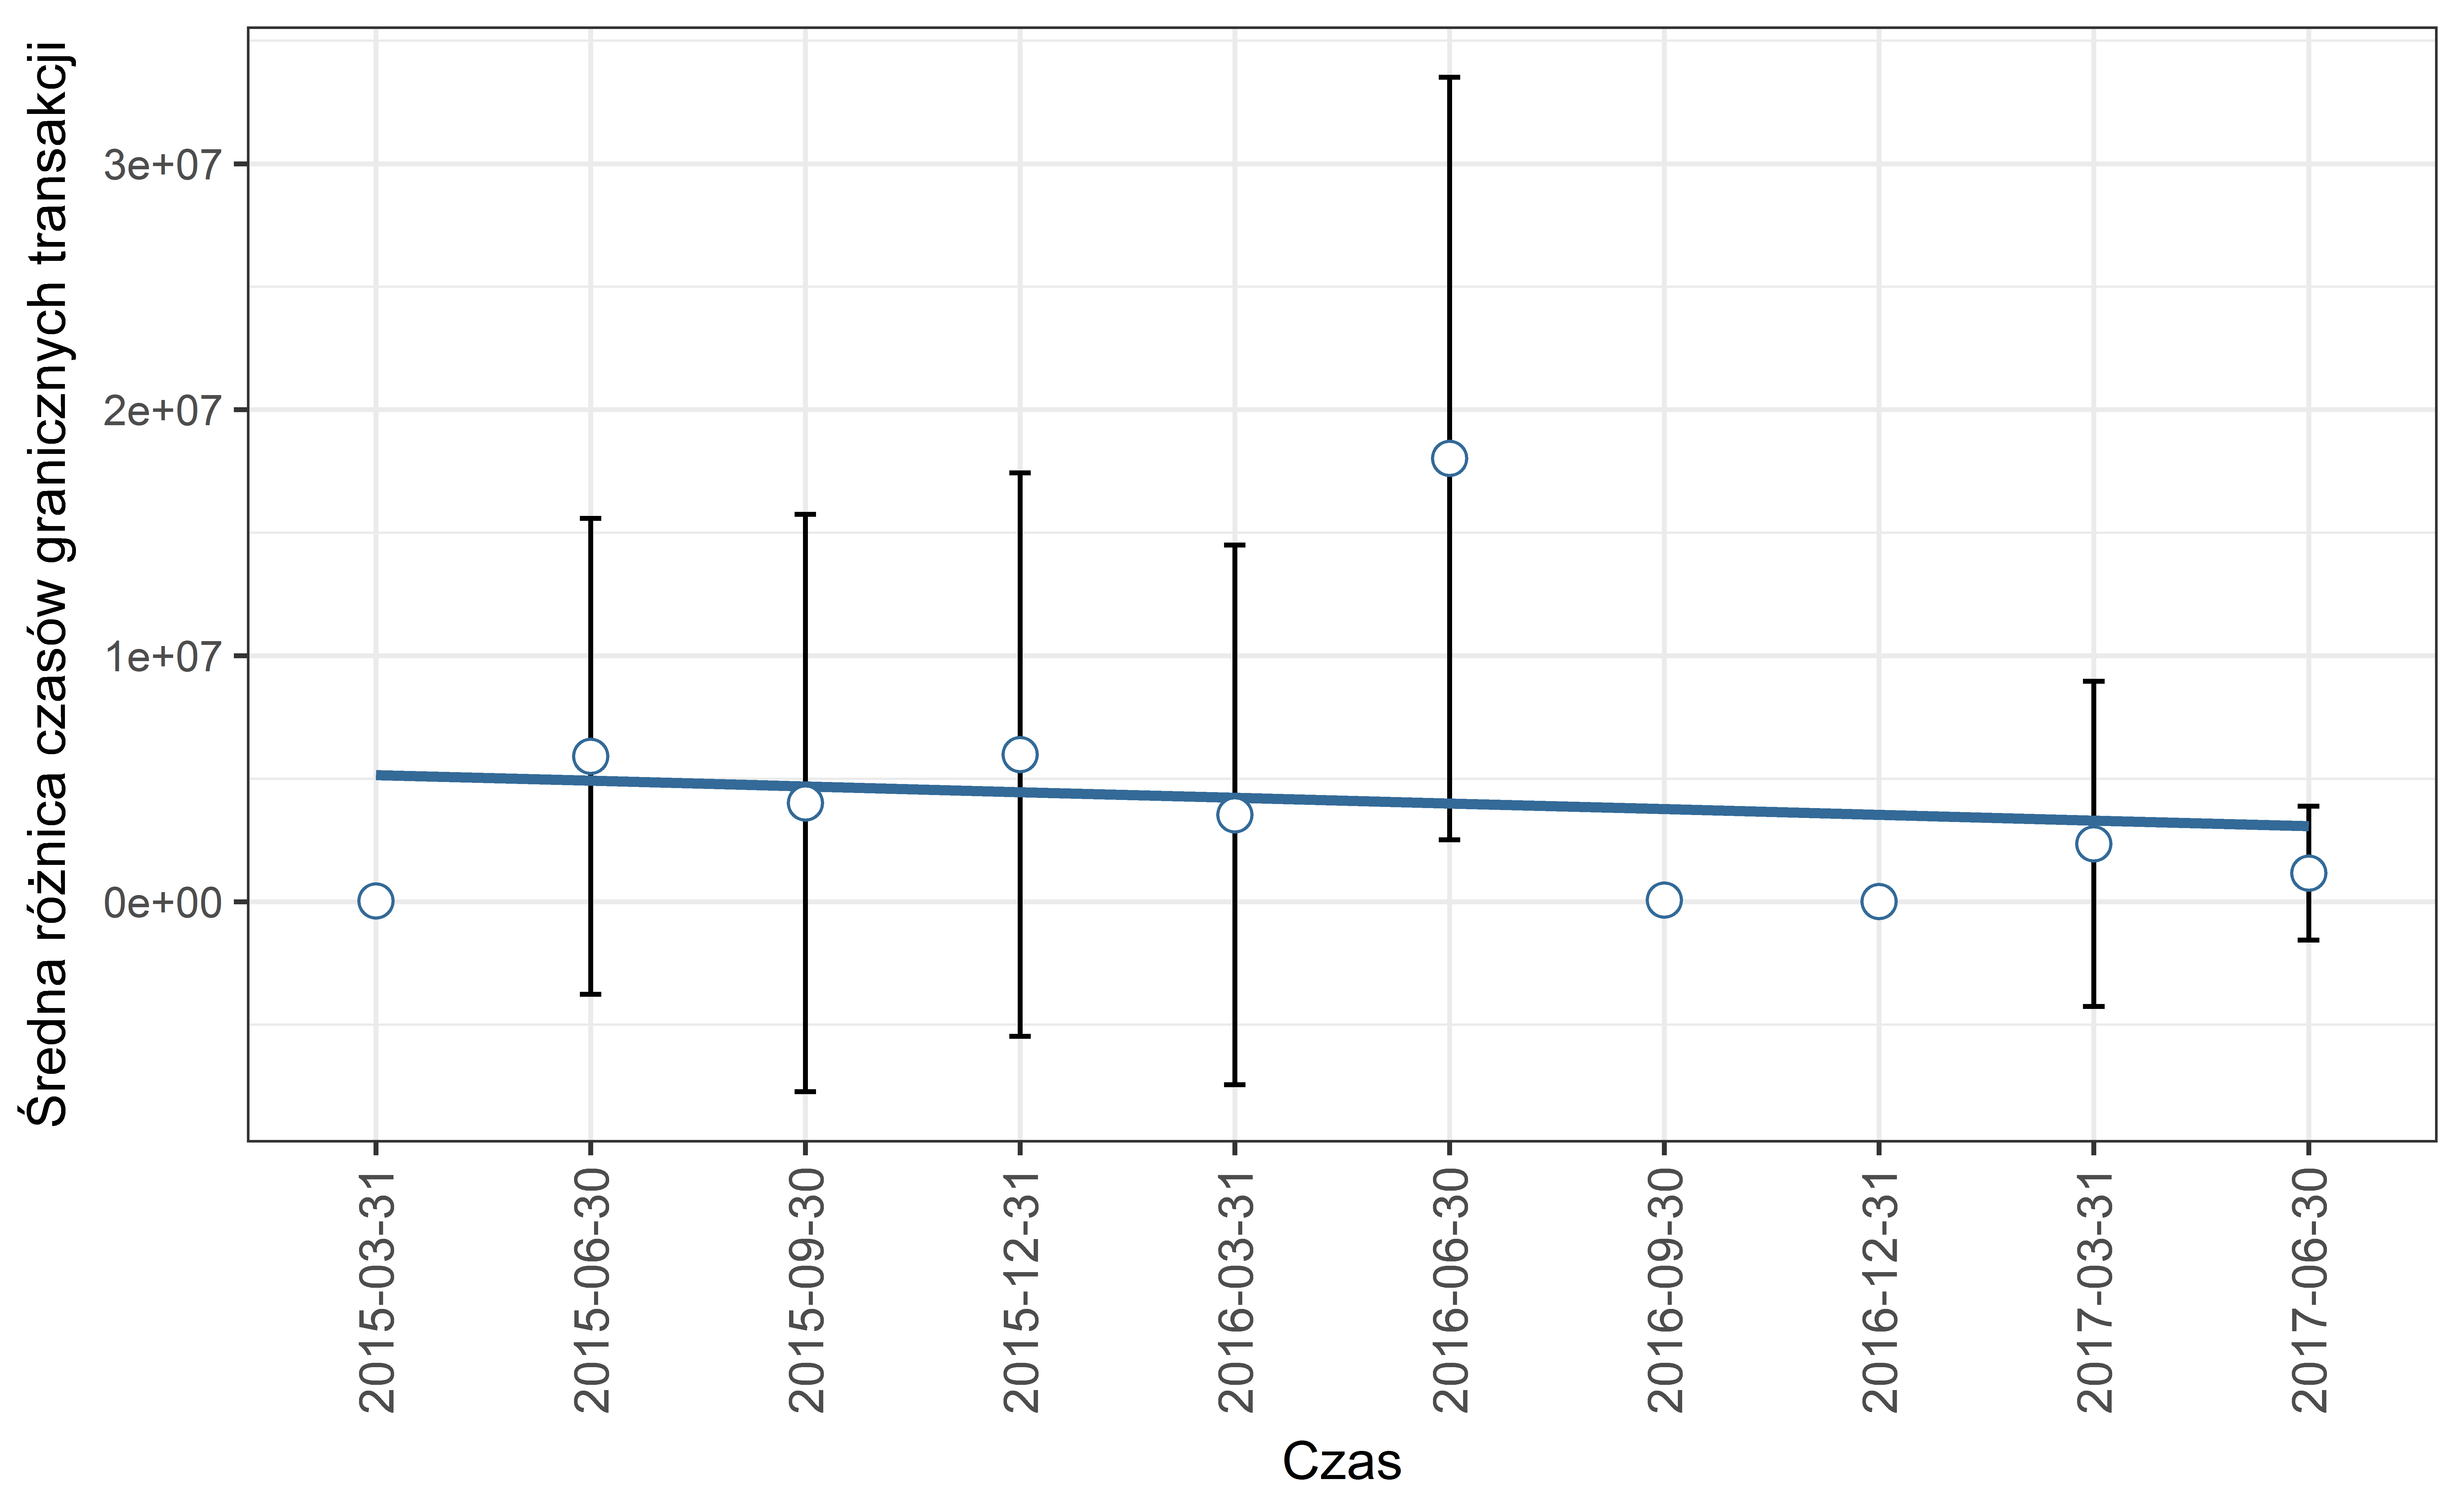
\includegraphics[width=\sizequadsda\textwidth]{pictures/czas_graniczny/czas_graniczny_sda.png}
  		  \end{minipage} 
\end{frame}


\begin{frame}
 \frametitle{Wnioski}
 \framesubtitle{}
 \begin{itemize}
 \item[1.] {\justifying{Sieć Bitcoin jest bardzo złożoną, dynamiczną i szybko rozwijającą się siecią.}\par} 
 \item[2.] {\justifying{Gęstość sieci rośnie, co w odniesieniu do jej specyfiki oznacza coraz większą ilość zlecanych transakcji, powstawanie dużej ilości nowych adresów oraz wzrost realizowanych transakcji pomiędzy różnymi uczestnikami sieci.}\par}
 \item[3.] {\justifying{Rosnąca ilość wykonywanych transakcji powoduje spadek istotności pojedynczej transakcji w całej sieci.}\par}
 \item[4.] {\justifying{Właściwości sieci nie są stałe w~jednym okresie, a~zależeć mogą od aktywności poszczególnych uczestników, dlatego też ilość połączeń pomiędzy transakcjami może być bardzo zróżnicowana.}\par}

  \end{itemize}
\end{frame}

\begin{frame}
 \frametitle{Wnioski}
 \framesubtitle{}
 \begin{itemize}
  \item[5.] {\justifying{Wartość większości transakcji nie przekracza 100 bitcoinów, a~zazwyczaj są to małe przekazy środków pomiędzy klientami sieci.}\par}
 \item[6.] {\justifying{Badanie ilości bloków potrzebnych do odnalezienia 100 tysięcy połączeń, w~powiązaniu z~analizą średniej różnicy czasów kolejnych transakcji oraz różnicy czasów transakcji granicznych jednoznacznie wskazuje na zwiększające się tempo rozwoju badanej sieci.}\par}
 \item[7.] {\justifying{Analiza znaczących wartości transakcji pozwoliła na powiązanie okresów z wzmożoną aktywnością giełd.}\par}
  \end{itemize}
\end{frame}

\begin{frame}
	\frametitle{Przyszłe kierunki badań}
	\justifying Kontynuacją niniejszej pracy mogłoby być stworzenie klasyfikatora dla adresów Bitcoin pozwalającego na identyfikację adresów należących, na przykład, do giełd. 
\begin{itemize}
\item {\justifying{Giełdy publikują posiadane adresy Bitcoin.}\par}
	\item {\justifying{Możliwe jest stworzenie prób rozpoczynających się od transakcji wykonanych z adresów giełd.}\par}
	\item {\justifying{Analiza prób, za pomocą metod użytych w niniejszej pracy, pozwoliłaby na określenie zakresów wartości danych właściwości, a to w efekcie umożliwiłoby budowę klasyfikatora.}\par}
\end{itemize}
	
\end{frame}

\begin{frame}
	\frametitle{}
	\centering
	Dziękuję za uwagę!
\end{frame}

\end{document}